\documentclass[11pt, a4paper, oneside]{Thesis} % Paper size, default font size and one-sided paper
\usepackage{floatrow}
\floatsetup[table]{capposition=top}
\usepackage{textcomp}
\usepackage{wrapfig}
\usepackage{lscape}
\usepackage{rotating}
\usepackage{graphicx}
\usepackage{caption}
\usepackage{amsmath}
\usepackage{upgreek}
\usepackage{gensymb}
\usepackage{csquotes}
\usepackage{pdfpages}
\usepackage{notoccite}
\usepackage{tikz}
\usepackage{pgfplots}
\pgfplotsset{compat=1.17}
\usetikzlibrary{positioning, arrows.meta, shapes.geometric, fit, calc}
\renewcommand{\chapterautorefname}{Chapter} % Forces capital "Chapter"
%\usepackage[open]{bookmark}

% acronyms
\usepackage{acronym}
\usepackage{array}
\newcolumntype{L}{>{\centering\arraybackslash}m{3cm}}

%\usepackage[acronym]{glossaries}
% prints author names as small caps


\makeatletter
\AtBeginDocument{%
  \renewcommand*{\AC@hyperlink}[2]{%
    \begingroup
      \hypersetup{hidelinks}%
      \hyperlink{#1}{#2}%
    \endgroup
  }%
}
\makeatother





%\usepackage{subcaption} %incompatible with subfig
\graphicspath{{Pictures/}} % Specifies the directory where pictures are stored
\usepackage[square, numbers]{natbib} % Use the natbib reference package - read up on this to edit the reference style; if you want text (e.g. Smith et al., 2012) for the in-text references (instead of numbers), remove 'numbers' v

\hypersetup{urlcolor=black, colorlinks=true} % Colors hyperlinks in blue - change to black if annoyingv`
\title{\ttitle} % Defines the thesis title - don't touch this

\begin{document}
\makeatletter
\renewcommand*{\NAT@nmfmt}[1]{\textsc{#1}}
\makeatother

% prints author names as small caps


\frontmatter % Use roman page numbering style (i, ii, iii, iv...) for the pre-content pages

\setstretch{1.6} % Line spacing of 1.6 (double line spacing)

% Define the page headers using the FancyHdr package and set up for one-sided printing
\fancyhead{} % Clears all page headers and footers
\rhead{\thepage} % Sets the right side header to show the page number
\lhead{} % Clears the left side page header

\pagestyle{fancy} % Finally, use the "fancy" page style to implement the FancyHdr headers

\newcommand{\HRule}{\rule{\linewidth}{0.5mm}} % New command to make the lines in the title page

% PDF meta-data
\hypersetup{pdftitle={\ttitle}}
\hypersetup{pdfsubject=\subjectname}
\hypersetup{pdfauthor=\authornames}
\hypersetup{pdfkeywords=\keywordnames}

%----------------------------------------------------------------------------------------
%	TITLE PAGE
%----------------------------------------------------------------------------------------

\begin{titlepage}
\begin{center}

\HRule \\[0.4cm] % Horizontal line
{\huge \bfseries \ttitle}\\[0.4cm] % Thesis title
\HRule \\[1.5cm] % Horizontal line
 
\large \textit{A thesis submitted in fulfilment of the requirements\\ for the degree of \degreename}\\[0.3cm] % University requirement text
\textit{by}\\[0.4cm]
\authornames \\



\vfill
% NOTE: Place the institute logo at Pictures/IIT_Jammu_Logo.png and
% uncomment the figure below before final submission.
% \begin{figure}[hb]
%   \centering
%   \includegraphics[width=0.55\linewidth]{Pictures/IIT_Jammu_Logo.png}
% \end{figure}

\DEPTNAME\\ % Research group name and department name
\textsc{ \UNIVNAME}\\[1.5cm] % University name
\large \today\\[2cm] % Date


\end{center}

\end{titlepage}

%----------------------------------------------------------------------------------------
%	DECLARATION PAGE
%	Your institution may give you a different text to place here
%----------------------------------------------------------------------------------------

\Declaration{\addtocontents{toc}{\vspace{1em}}} % Add a gap in the Contents, for aesthetics
\setcounter{page}{2}

\begin{minipage}{\textwidth}
    
    It is certified that the work contained in this thesis entitled \textbf{\enquote{\ttitle}} by \textbf{\authornames} has been carried out under my supervision and that it has not been submitted elsewhere for a degree.
        
\end{minipage}

\vspace{20.00mm}

\begin{minipage}{0.49\textwidth}
		\begin{flushleft}
			{\supnameA\\
			Professor\\
			\deptname\\
			\univname}
		\end{flushleft}
\end{minipage}
\vfill
\clearpage % Start a new page
\StudentDeclaration{\addtocontents{toc}{\vspace{1em}}} % Add a gap in the Contents, for aesthetics

This is to certify that the thesis titled \textbf{``\ttitle''} has been authored by me. It presents the research conducted by me under the supervision of \textbf{\supnameA}.\par

To the best of my knowledge, it is an original work, both in terms of research content and narrative, and has not been submitted elsewhere, in part or in full, for a degree. Further, due credit has been attributed to the relevant state-of-the-art and collaborations with appropriate citations and acknowledgments, in line with established norms and practices.\\ [2cm]
\begin{minipage}{.5\textwidth}
		\begin{flushleft}
			{\authornames\\ Roll No. 2024OVL1079 \\
			\normalsize{\href{https://www.iitjammu.ac.in/cep/}{CEP Department}\\
			\univname}}
		\end{flushleft}
\end{minipage}
\vfill

\clearpage % Start a new page
%----------------------------------------------------------------------------------------
%	ABSTRACT PAGE
%----------------------------------------------------------------------------------------

%\addtotoc{Abstract} % Add the "Abstract" page entry to the Contents
\lhead{\emph{Abstract}}

\abstract{\addtocontents{toc}{\vspace{1em}} % Add a gap in the Contents, for aesthetics

Peripheral Component Interconnect Express (PCIe) is the dominant interconnect for attaching high-performance peripherals to a host processor, and Direct Memory Access (DMA) engines built on top of the AMBA AXI4 and AXI4-Stream protocols are the standard mechanism by which such peripherals move data to and from host memory without processor intervention. While this combination delivers high sustained throughput for large, bulk transfers, its behaviour for small packets -- tens to a few hundred bytes, as generated by network interface cards, sensor front-ends, and low-latency control-plane traffic -- is comparatively poorly characterised. Each transfer incurs largely size-independent fixed costs: PCIe transaction-layer packet framing and credit accounting, and DMA descriptor fetch and doorbell signalling. For small payloads these fixed costs are amortised over very few bytes, so per-byte latency and effective throughput degrade sharply as packet size shrinks.

This thesis develops a cycle-accurate latency model of a PCIe-AXI DMA streaming datapath and uses it to quantify, and partially mitigate, this small-packet inefficiency. A seven-stage behavioural pipeline -- \texttt{pcie\_model}, \texttt{dma\_model}, an AXI-memory-mapped-to-AXI-Stream adapter, a parameterised AXI-Stream FIFO, a packet-batching unit, a stream sink, and a hardware latency monitor -- is implemented in synthesisable SystemVerilog and driven by a self-checking testbench in the Vivado xsim simulator. Packet-size-dependent PCIe and DMA delay models are derived analytically from published transaction-layer and descriptor-processing overheads and validated against per-packet latency measurements taken directly from the simulated hardware, with the latency monitor decomposing every measurement into its PCIe, DMA, and residual pipeline contributions.

Simulation results for packet sizes from 64~B to 4~KB show per-byte efficiency rising from 0.90~B/cycle at 64~B to 1.58~B/cycle at 4~KB, confirming that fixed per-packet overhead, not link or memory bandwidth, dominates small-transfer latency. To address this, a small-packet batching unit is designed and evaluated: coalescing four 64~B packets into a single 256~B frame reduces total transfer latency from 284 cycles (four packets sent independently) to 230 cycles, a 19\% reduction, by amortising one PCIe and DMA overhead charge across four packets instead of paying it four times. A complementary FIFO-depth sweep under a rate-limited consumer shows that buffer depth governs how much back-pressure headroom the datapath has and how early it engages, but does not by itself change steady-state single-flow completion latency once the consumer's drain rate becomes the bottleneck -- a distinction that is often conflated in informal DMA sizing guidelines. Together, these results provide a validated, reusable latency model and a concrete, RTL-proven optimisation for small-packet PCIe-AXI DMA transfers, along with a measurement infrastructure that can be extended to other datapath configurations and workloads.

}





%----------------------------------------------------------------------------------------
%	Declaration Page
%----------------------------------------------------------------------------------------



%----------------------------------------------------------------------------------------
%	ACKNOWLEDGEMENTS
%----------------------------------------------------------------------------------------
\clearpage % Start a new page
\setstretch{1.3} % Reset the line-spacing to 1.3 for body text (if it has changed)
\lhead{\emph{Acknowledgements}}
\acknowledgements{\addtocontents{toc}{\vspace{1em}} % Add a gap in the Contents, for aesthetics

I would like to express my sincere gratitude to my supervisor, \supnameA, for his guidance, patience, and constructive criticism throughout the course of this thesis. His feedback at every stage, from the initial formulation of the problem to the interpretation of the final latency results, was instrumental in shaping the direction and rigour of this work.

I am thankful to the Department of Continuing Education Program (CEP) and to the Indian Institute of Technology Jammu for providing the academic environment, computing resources, and access to the Vivado design suite that made the simulation-based study reported here possible.

I would also like to thank my colleagues and peers in the M.Tech program for the many useful discussions on AXI-based system design and PCIe architecture that helped refine the ideas presented in this thesis.

Finally, I am deeply grateful to my family for their constant encouragement, patience, and support throughout this program.

}
\clearpage % Start a new page

%----------------------------------------------------------------------------------------
%	LIST OF CONTENTS/FIGURES/TABLES PAGES
%----------------------------------------------------------------------------------------

\pagestyle{fancy} % The page style headers have been "empty" all this time, now use the "fancy" headers as defined before to bring them back

\lhead{\emph{Contents}} % Set the left side page header to "Contents"
\tableofcontents % Write out the Table of Contents

\lhead{\emph{List of Figures}} % Set the left side page header to "List of Figures"
\listoffigures % Write out the List of Figures

\lhead{\emph{List of Tables}} % Set the left side page header to "List of Tables"
\listoftables % Write out the List of Tables

%----------------------------------------------------------------------------------------
%	ABBREVIATIONS
%----------------------------------------------------------------------------------------




\clearpage % Start a new page

\setstretch{1.5} % Set the line spacing to 1.5, this makes the following tables easier to read

\lhead{\emph{Abbreviations}} % Set the left side page header to "Abbreviations"

\chapter*{Abbreviations}
\addtotoc{Abbreviations}
\begin{acronym}[AXI4-Stream] % Give the longest label here so that the list is nicely aligned
\acro{PCIe}{Peripheral Component Interconnect Express}
\acro{AXI}{Advanced eXtensible Interface}
\acro{AXI4}{Advanced eXtensible Interface, version 4}
\acro{AXI4-Stream}{Advanced eXtensible Interface 4 Stream}
\acro{FPGA}{Field-Programmable Gate Array}
\acro{AMBA}{Advanced Microcontroller Bus Architecture}
\acro{DMA}{Direct Memory Access}
\acro{TLP}{Transaction Layer Packet}
\acro{FIFO}{First-In First-Out}
\acro{FWFT}{First-Word Fall-Through}
\acro{FSM}{Finite State Machine}
\acro{RTL}{Register-Transfer Level}
\acro{HDL}{Hardware Description Language}
\acro{IP}{Intellectual Property}
\acro{SoC}{System-on-Chip}
\acro{NIC}{Network Interface Card}
\acro{DDR}{Double Data Rate}
\acro{BRAM}{Block Random Access Memory}
\acro{MM2S}{Memory-Mapped to Stream}
\acro{S2MM}{Stream to Memory-Mapped}
\acro{DUT}{Design Under Test}
\acro{TB}{Testbench}
\acro{MTP}{Master's Thesis Project}
\acro{PIO}{Programmed Input/Output}
\acro{RC}{Root Complex}
\acro{EP}{Endpoint}
\acro{QoS}{Quality of Service}
\acro{NVMe}{Non-Volatile Memory Express}
\acro{RDMA}{Remote Direct Memory Access}
\acro{MHz}{Megahertz}
\end{acronym}





%----------------------------------------------------------------------------------------
%	PHYSICAL CONSTANTS/OTHER DEFINITIONS
%----------------------------------------------------------------------------------------
%
% \clearpage % Start a new page

% \lhead{\emph{Physical Constants}} % Set the left side page header to "Physical Constants"

% \listofconstants{lrcl} % Include a list of Physical Constants (a four column table)
% {
% Speed of Light & $c$ & $=$ & $2.997\ 924\ 58\times10^{8}\ \mbox{ms}^{-\mbox{s}}$ (exact)\\
% % Constant Name & Symbol & = & Constant Value (with units) \\
% }

%----------------------------------------------------------------------------------------
%	SYMBOLS
%----------------------------------------------------------------------------------------

\clearpage % Start a new page

\lhead{\emph{Symbols}} % Set the left side page header to "Symbols"

\listofnomenclature{lll} % Include a list of Symbols (a two column table)
{
% Symbol & Name & Unit \\
$L_{PCIe}$ & PCIe transaction-layer delay & cycles \\
$L_{DMA}$  & DMA engine delay & cycles \\
$L_{tot}$  & End-to-end packet latency & cycles \\
$T_{base}$ & PCIe fixed (per-TLP) base latency & cycles \\
$T_{dw}$   & PCIe per-DWORD latency & cycles/DWORD \\
$T_{setup}$& DMA descriptor setup latency & cycles \\
$S$        & Packet payload size & bytes \\
$W$        & AXI data bus width & bytes/beat \\
$N$        & Number of packets per batch & -- \\
$D$        & AXI-Stream FIFO depth & beats \\
$\eta$     & Effective transfer efficiency ($S/L_{tot}$) & bytes/cycle
}

\ListofPublications{\addtocontents{toc}{\vspace{1em}} % Add a gap in the Contents, for aesthetics

\textbf{Publications from Thesis}

No publications had resulted from this thesis at the time of submission.

}









% \\[2cm]


%\vfill{}


\clearpage % Start a new page





\setstretch{1.3} % Return the line spacing back to 1.3
%
\pagestyle{empty} % Page style needs to be empty for this page
%
\dedicatory{Dedicated to family.
} % Dedication text
%
\addtocontents{toc}{\vspace{2em}} % Add a gap in the Contents, for aesthetics

%----------------------------------------------------------------------------------------
%	THESIS CONTENT - CHAPTERS
%----------------------------------------------------------------------------------------

\mainmatter % Begin numeric (1,2,3...) page numbering

\pagestyle{fancy} % Return the page headers back to the "fancy" style

% Include the chapters of the thesis as separate files from the Chapters folder
% Uncomment the lines as you write the chapters

% Chapter 1

\chapter{Introduction}

\label{Chapter1}

\lhead{Chapter 1. \emph{Introduction}}

%----------------------------------------------------------------------------------------
%	SECTION: BACKGROUND
%----------------------------------------------------------------------------------------

\section{Background}
\label{sec:ch1_background}

\ac{PCIe} has become the standard interconnect for attaching high-performance peripherals -- network interface cards, solid-state storage controllers, accelerators, and custom \ac{FPGA}-based devices -- to a host processor \cite{pcisig2017base, budruk2004pcie}. Almost every such peripheral moves bulk data to and from host memory using a \ac{DMA} engine rather than processor-driven \ac{PIO}, because \ac{DMA} allows large transfers to proceed without consuming host CPU cycles for every word moved. On the \ac{FPGA} or \ac{SoC} fabric side of the interconnect, these \ac{DMA} engines are almost universally built around the \ac{AMBA} \ac{AXI} family of on-chip bus protocols, with the \ac{AXI4-Stream} variant used specifically for the unidirectional, back-pressure-aware data streams that connect a \ac{DMA} engine to downstream processing logic \cite{arm2021axi, arm2010axistream}.

A complete host-to-device or device-to-host transfer over such a datapath therefore crosses two distinct protocol domains. On the PCIe side, data is carried inside \acp{TLP}, each of which carries a fixed-size header, is subject to credit-based flow control, and incurs round-trip latency for link-level acknowledgement. On the AXI side, a DMA engine such as the AMD-Xilinx AXI DMA \ac{IP} \cite{xilinx2021axidma} or the integrated PCIe block on UltraScale+ devices \cite{xilinx2021pcieintblock} translates between memory-mapped burst reads/writes and byte-enabled AXI4-Stream beats, typically after first fetching a descriptor that specifies the source address, destination address, and transfer length for the operation. Both of these mechanisms -- TLP framing and descriptor fetch -- impose a processing cost that is largely independent of how many bytes are actually being moved.

For large transfers (multi-kilobyte and above), this fixed cost is negligible relative to the time spent moving payload bytes, and the datapath approaches its peak link bandwidth. For small transfers, however, the same fixed cost dominates: a 64-byte packet pays essentially the same TLP-header and descriptor-setup penalty as a 4096-byte packet, so its effective throughput and per-byte latency are far worse. Such small, latency-sensitive transfers are common in practice -- network packet forwarding, sensor telemetry, control-plane messages, and lock-step accelerator hand-offs all routinely move payloads well under one kilobyte -- which makes the small-packet regime an important, if under-examined, corner of PCIe-AXI DMA system design.

%----------------------------------------------------------------------------------------
%	SECTION: MOTIVATION
%----------------------------------------------------------------------------------------

\section{Motivation}
\label{sec:ch1_motivation}

Vendor documentation for AXI DMA and PCIe integrated-block IP cores specifies functional behaviour, register maps, and peak bandwidth figures, but rarely quantifies how the combined PCIe + DMA + AXI-Stream pipeline behaves as a function of packet size, nor does it typically expose a validated, cycle-level breakdown of where the latency of a single small transfer is actually spent. System architects sizing a design are consequently left to over-provision buffering, guess at achievable small-packet throughput, or discover the fixed-overhead penalty only after silicon or FPGA bring-up. Prior systems work on PCIe performance, such as the end-host networking characterisation of Neugebauer~et~al.~\cite{neugebauer2018pcie}, confirms empirically that small-transfer PCIe performance is dominated by per-descriptor and per-TLP overheads rather than raw link bandwidth, but that work characterises commodity NIC/host systems as a whole rather than providing an open, instrumented, packet-size-parameterised RTL model that a designer can simulate, modify, and re-measure.

A closely related body of work in operating-systems networking establishes that batching or coalescing many small, fixed-overhead events into fewer, larger ones is a general and effective way to amortise per-event cost -- interrupt coalescing to avoid receive livelock \cite{mogul1997livelock} and hardware interrupt-moderation timers on commodity NICs \cite{intel2003moderation} are the classic examples. The same amortisation principle should, in principle, apply directly to PCIe-AXI DMA packet transfers: if the fixed cost is paid once per TLP/descriptor rather than once per application-level packet, small-packet efficiency should improve substantially. However, this transfer of a software networking technique into an RTL DMA datapath, together with a quantitative before/after measurement of the improvement it yields, does not appear to be addressed by existing IP-core documentation or the PCIe performance literature surveyed in \autoref{Chapter2}.

This gap motivates the present thesis: to build a cycle-accurate, parameterised model of a PCIe-AXI DMA streaming pipeline; to use it to measure, rather than estimate, how end-to-end latency and per-byte efficiency vary with packet size; and to design, implement, and evaluate a packet-batching mechanism as a concrete mitigation, all within a synthesisable RTL testbed that can be re-run under different configurations.

%----------------------------------------------------------------------------------------
%	SECTION: PROBLEM STATEMENT
%----------------------------------------------------------------------------------------

\section{Problem Statement}
\label{sec:ch1_problem}

Given a PCIe-AXI DMA streaming datapath composed of a PCIe transaction layer, a descriptor-driven DMA engine, an AXI-Stream buffering stage, and a consumer, this thesis addresses the following problem: \emph{quantify the end-to-end latency and effective throughput of the datapath as a function of packet size, decompose that latency into its PCIe, DMA, and buffering contributions, and design an RTL-level optimisation that measurably improves small-packet efficiency without modifying the underlying PCIe or AXI protocols.}

This is decomposed into four concrete sub-problems, each addressed in a later chapter:
\begin{enumerate}
    \item \textbf{Modeling.} Derive closed-form, packet-size-dependent latency expressions for the PCIe transaction layer and the DMA engine, grounded in the fixed-overhead-plus-linear-transfer structure documented for real TLP framing and descriptor processing (\autoref{Chapter3}).
    \item \textbf{Implementation.} Realise these models, together with an AXI-Stream FIFO, a batching unit, and a hardware latency-measurement block, as synthesisable SystemVerilog RTL that can be simulated cycle-accurately (\autoref{Chapter4}, \autoref{Chapter5}).
    \item \textbf{Measurement.} Build a self-checking testbench that injects packets of varying size and configuration into the RTL pipeline and measures per-packet latency directly in hardware, not via a software proxy (\autoref{Chapter6}).
    \item \textbf{Optimisation and evaluation.} Implement a small-packet batching unit, and quantify its latency and efficiency benefit against the un-batched baseline, together with a study of how AXI-Stream FIFO depth affects buffering headroom under a rate-limited consumer (\autoref{Chapter7}).
\end{enumerate}

%----------------------------------------------------------------------------------------
%	SECTION: OBJECTIVES
%----------------------------------------------------------------------------------------

\section{Objectives of the Thesis}
\label{sec:ch1_objectives}

The specific objectives pursued in this work are:

\begin{enumerate}
    \item To develop an analytical latency model for a PCIe transaction layer and a descriptor-based DMA engine, expressing per-packet delay as a fixed base term plus a term proportional to packet size.
    \item To design and implement, in synthesisable SystemVerilog, a seven-stage behavioural pipeline (\texttt{pcie\_model}, \texttt{dma\_model}, an AXI memory-mapped-to-stream adapter, a parameterised AXI-Stream FIFO, a batching unit, a stream sink, and a hardware latency monitor) that reproduces this latency behaviour cycle-accurately.
    \item To build a directed SystemVerilog testbench that exercises the pipeline across a representative range of packet sizes (64~B to 4~KB) and configurations, and to validate the hardware-measured latency against the analytical model.
    \item To design a small-packet batching mechanism that coalesces multiple small packets into a single larger AXI-Stream frame before it reaches the PCIe/DMA overhead-paying stages, and to quantify the resulting latency and efficiency improvement relative to the un-batched baseline.
    \item To characterise the effect of AXI-Stream FIFO depth on buffering headroom and back-pressure behaviour under both an always-ready and a rate-limited (stalling) consumer, and to correctly distinguish buffering headroom from steady-state throughput.
\end{enumerate}

%----------------------------------------------------------------------------------------
%	SECTION: ORGANIZATION OF THE THESIS
%----------------------------------------------------------------------------------------

\section{Organization of the Thesis}
\label{sec:ch1_organization}

The remainder of this thesis is organised as follows. \autoref{Chapter2} reviews prior work on PCIe performance characterisation, AXI-based DMA architectures, and overhead-amortisation techniques such as interrupt and transfer coalescing, and identifies the specific research gap this thesis addresses. \autoref{Chapter3} presents the background material -- the PCIe transaction layer, the AMBA AXI4 and AXI4-Stream protocols, descriptor-based DMA operation, and the queueing-theoretic notion of fixed-plus-proportional service time -- needed to justify the latency model used later. \autoref{Chapter4} describes the system architecture of the implemented PCIe-AXI DMA streaming pipeline, module by module, together with the inter-stage AXI-Stream signalling conventions. \autoref{Chapter5} details the design and implementation methodology, including the finite-state-machine designs of the PCIe and DMA models, the batching-unit algorithm, and the hardware latency-monitor instrumentation. \autoref{Chapter6} describes the experimental setup: the Vivado xsim simulation flow, the testbench architecture, and the verification milestones completed during the project. \autoref{Chapter7} presents and analyses the simulation results -- baseline latency and efficiency versus packet size, the per-stage latency breakdown, the batching experiment, and the FIFO-depth sweep -- and discusses their implications. \autoref{Chapter8} concludes the thesis, summarising the research contributions, discussing the limitations of the present model, and outlining directions for future work.

% Chapter 2

\chapter{Literature Review}

\label{Chapter2}

\lhead{Chapter 2. \emph{Literature Review}}

This chapter looks at the four main areas that this thesis is based on: how well the PCIe protocol works, designing DMA architectures using AXI, ways to reduce overhead from systems and networking research, and modeling latency in on-chip interconnects using RTL and queueing theory. Then, in section 2, we identify the specific problem that this thesis aims to solve.

%----------------------------------------------------------------------------------------

\section{PCIe Protocol and Performance Characterisation}
\label{sec:ch2_pcie}

The \ac{PCIe} Base Specification \cite{pcisig2017base} defines a layered architecture -- transaction, data link, and physical layers -- in which application data is carried inside \acp{TLP}. Every \ac{TLP} carries a fixed-size header (typically 12--16 bytes for memory requests), is subject to credit-based flow control between the transmitter and receiver, and its delivery is acknowledged at the data-link layer. Budruk~et~al.~\cite{budruk2004pcie} provide a detailed treatment of this layering and of the round-trip credit and acknowledgement mechanisms that contribute fixed, size-independent latency to every transaction, independent of the physical-layer transfer rate.

Here's a rewritten version of the input text in a more human-like tone, mimicking the style and structure of the provided human samples: When it comes to understanding how fixed-overhead behaviour works in real systems, there's surprisingly little research out there. One study by Neugebauer et al. did look at how PCIe performs in end-host networking on regular servers. They found that when it comes to small DMA transfers - the kind that's most relevant to packet-processing NICs - the throughput is actually determined by the number of separate PCIe transactions, rather than the total amount of data being transferred. To get close to the link bandwidth, they had to batch multiple descriptors or payloads per transaction. Now, their measurements were taken on actual production hardware, and they treated the NIC and host as a single unit - a black box, essentially. But what they didn't do was create a detailed model of the datapath that would show exactly how much of the overhead is due to the PCIe transaction layer, and how much is due to the DMA engine's descriptor processing. They also didn't provide a way to experimentally adjust the balance between these two factors. This is what motivated us to break down the system into smaller modules, as we'll see in Chapter 4 of this thesis.

%----------------------------------------------------------------------------------------

\section{AXI-Based DMA Architectures}
\label{sec:ch2_axi_dma}

On the fabric side of a PCIe endpoint, the \ac{AMBA} \ac{AXI4} and \ac{AXI4-Stream} protocols \cite{arm2021axi, arm2010axistream} are the de facto standard for connecting a DMA engine to on-chip processing logic. AXI4 defines a memory-mapped, burst-oriented protocol with independent address and data channels, while AXI4-Stream strips away addressing entirely in favour of a simple, back-pressured (\texttt{tvalid}/\texttt{tready}) beat-by-beat handshake with sideband fields (\texttt{tlast}, \texttt{tkeep}, \texttt{tuser}, \texttt{tid}) that this thesis reuses directly to carry per-packet size and identity information through the pipeline (\autoref{sec:ch4_sideband}).

Commercial DMA engines, like the AMD-Xilinx AXI DMA and the DMA/bridge logic in the UltraScale+ PCIe endpoint block, use a descriptor-ring model to operate. Here's how it works: the host or an on-chip processor writes a descriptor with details like source address, destination address, and length to a ring buffer in memory. Then, it signals the engine using a doorbell register or interrupt. The engine has to fetch and parse this descriptor, which is a memory or PCIe transaction with its own latency, before it can start moving the payload. The product guides for these cores provide information on register maps, supported burst lengths, and peak throughput figures. However, they don't model descriptor-fetch latency as a function of transfer size, treating it as an implementation detail instead. In contrast, this thesis's DMA model makes the fixed descriptor-processing cost a clear, parameterized quantity, called SETUP CYCLES. This allows us to isolate and measure its contribution to small-packet latency. By doing so, we can better understand the impact of this cost on the overall performance of the DMA engine. For instance, when transferring small packets, the descriptor-fetch latency can become a significant bottleneck. By explicitly modeling this cost, we can identify areas for optimization and improve the overall efficiency of the DMA engine. This is particularly important in applications where low latency is crucial, such as in real-time systems or high-performance computing. In summary, the descriptor-ring model used by commercial DMA engines has its own set of challenges, particularly when it comes to descriptor-fetch latency. By making this cost explicit and parameterized, we can gain a better understanding of its impact on performance and identify opportunities for improvement. This can lead to more efficient and effective DMA engines, which are essential in a wide range of applications.

%----------------------------------------------------------------------------------------

\section{Overhead Amortisation and Batching Techniques}
\label{sec:ch2_batching}

The idea behind the batching unit in this thesis is simple: combining many small events into fewer, larger ones can make them more efficient. This concept has been around for a while in systems and networking research, but it's usually applied in software or at a higher level, not directly in hardware like an RTL DMA datapath. For example, Mogul and Ramakrishnan found that when a network receives a lot of packets, handling each one with an individual interrupt can cause problems and slow things down. They showed that by polling and combining interrupts, so that multiple packets are handled at once, the system can recover and work more efficiently. This is because the fixed cost of handling each interrupt is spread out over many packets, making it more cost-effective. Later, network interface controllers started including hardware timers that could delay interrupts until a certain number of packets had arrived or a timeout had expired. This added a bit of latency to each packet, but it greatly reduced the overhead of handling each packet individually. By trading off a small amount of extra delay for a big reduction in overhead, these controllers could handle more packets and improve overall performance. This approach has been used in various forms, but the key idea is the same: by combining small events into larger ones, we can make systems more efficient and improve their performance. In the context of this thesis, the batching unit applies this principle to the RTL DMA datapath, aiming to reduce overhead and improve efficiency in a similar way.

These methods work at the point where the hardware and the operating system meet, combining signals that interrupt the system rather than the actual movement of data. The concept of using the same principle a step further down - combining many small packets of data into one big frame before they get to the parts of the system that add a fixed cost, and then measuring how much this improves things directly in a simulation - is what this project is about. It puts this idea into action with a part called the batching unit and checks how well it works with real numbers.

%----------------------------------------------------------------------------------------

\section{Latency Modeling of Interconnects}
\label{sec:ch2_latency_modeling}

Analytically, the behaviour this thesis is concerned with -- a service time made up of a fixed component plus a component proportional to the size of the job being served -- is a standard construction in queueing theory. Kleinrock's treatment of queueing systems \cite{kleinrock1975queueing} formalises service-time models of exactly this fixed-plus-proportional form and their consequences for waiting time and utilisation, and provides the conceptual basis for the closed-form PCIe and DMA delay expressions derived in \autoref{sec:ch3_latency_model}. However, classical queueing analysis models the service discipline abstractly; it does not, by itself, validate whether a specific RTL implementation of a specific protocol actually exhibits the assumed fixed-plus-proportional behaviour, or by how much a specific mitigation (such as batching) improves it for a specific packet-size distribution. Closing that gap between an analytical model and a cycle-accurate, simulatable hardware implementation -- built using standard SystemVerilog RTL practice \cite{ieee2017systemverilog} and simulated with an industrial simulator \cite{xilinx2022vivadosim} -- is the methodological contribution of this thesis.

%----------------------------------------------------------------------------------------

\section{Research Gap}
\label{sec:ch2_gap}

Synthesising the four areas above, three gaps recur:

\begin{enumerate}
\item \textbf{No open, parameterised, per-stage latency model.} PCIe performance studies \cite{neugebauer2018pcie} characterise small-transfer inefficiency empirically on commodity hardware, but as a single opaque number rather than a model that separately attributes latency to the PCIe transaction layer versus the DMA descriptor-processing stage. Vendor IP documentation \cite{xilinx2021axidma, xilinx2021pcieintblock} specifies the mechanisms that create this overhead (TLP framing, descriptor fetch) but does not quantify it as a function of packet size.
* **No use of batching at the RTL level for PCIe-AXI DMA transfers**. The idea of coalescing is already used for network interrupts, as seen in previous work, but applying this concept directly to an AXI-Stream DMA pipeline is not well documented. This means merging small packets into a larger frame before the PCIe/DMA overhead, and then measuring how this affects latency at the cycle level, is not something you can find in the literature or vendor documentation.
* There's no proven connection between the theoretical model and actual hardware measurements. The fixed-plus-proportional service models are commonly used in queueing theory, as seen in Kleinrock's work, but we need to know if a real PCIe-AXI DMA RTL pipeline really works this way. We also want to understand how much a solution like batching can improve it. To do this, we need a version of the pipeline that can be measured and simulated, which currently doesn't exist in the available research. This is a problem because it means we can't be sure if our theories are correct or how well our solutions will work in practice.
\end{enumerate}

This research tackles all three gaps at once. It starts by creating a detailed model of a PCIe-AXI DMA pipeline in Chapters 3 and 4, which takes into account the size of packets and how that affects latency. Then, in Chapter 5, it puts the coalescing principle into practice by adding a batching unit directly into the design. Finally, in Chapters 6 and 7, it checks how well the model works and measures the improvement that batching brings by using precise measurements from a hardware latency monitor built into the simulated design. 
% Chapter 3

\chapter{Background}

\label{Chapter3}

\lhead{Chapter 3. \emph{Background}}

This chapter presents the protocol and analytical background required to justify the latency model implemented later in the thesis. \autoref{sec:ch3_pcie} summarises the relevant parts of the PCIe transaction layer, \autoref{sec:ch3_axi} summarises the AMBA AXI4 and AXI4-Stream protocols, \autoref{sec:ch3_dma} describes descriptor-based DMA operation, and \autoref{sec:ch3_latency_model} combines these into the fixed-plus-proportional latency model used throughout the remainder of the thesis.

%----------------------------------------------------------------------------------------

\section{The PCIe Transaction Layer}
\label{sec:ch3_pcie}

\ac{PCIe} is a point-to-point, packet-switched interconnect organised as three layers: physical, data link, and transaction \cite{pcisig2017base}. Application-level reads and writes are carried as \acp{TLP} at the transaction layer. Every \ac{TLP} carries a header (12 or 16 bytes depending on addressing mode) that encodes the transaction type, requester ID, tag, address, and length, in addition to whatever payload it carries. Two mechanisms in this layering contribute latency that does not depend on payload size:

\begin{itemize}
    \item \textbf{Header and framing overhead.} Every TLP, regardless of payload size, must be assembled, have its header fields populated, and pass through link-layer framing (start/end control symbols, CRC) before transmission, and must be decoded and checked symmetrically at the receiver.
    \item \textbf{Credit-based flow control.} A PCIe transmitter may not send a TLP unless it holds sufficient flow-control credits, advertised by the receiver. For an idle or lightly loaded link, the first TLP of a transaction typically requires a credit round-trip before it can proceed, and for posted writes/completions a further acknowledgement may be pipelined behind it \cite{budruk2004pcie}.
\end{itemize}

Neither of these costs scales with the number of bytes in the payload; both are why a link that appears to run near its peak line rate for large bursts can appear far slower, per byte, for small ones. Beyond this fixed cost, transmission of the payload itself does scale with size: at a given link width and speed, moving $S$ bytes takes time proportional to $S$, i.e. proportional to the number of PCIe \emph{DWORDs} (4-byte units) the payload occupies, since PCIe headers and data paths are DWORD-aligned. This structure -- a fixed term plus a term proportional to $\lceil S/4 \rceil$ DWORDs -- is the basis for the PCIe delay model derived in \autoref{sec:ch3_latency_model}.

%----------------------------------------------------------------------------------------

\section{The AMBA AXI4 and AXI4-Stream Protocols}
\label{sec:ch3_axi}

On the fabric side of a PCIe endpoint, the \ac{AMBA} \ac{AXI4} protocol \cite{arm2021axi} provides a memory-mapped, burst-oriented interface with independent, decoupled address and data channels, and is the interface most on-chip DMA engines and memory controllers present to a bus fabric. \ac{AXI4-Stream} \cite{arm2010axistream} is a companion protocol that removes addressing entirely, retaining only a simple point-to-point, back-pressured data channel intended for continuous or packetised data movement between IP blocks. Its handshake and sideband signals, all of which are used directly by the datapath implemented in this thesis, are:

\begin{itemize}
    \item \texttt{tvalid} / \texttt{tready} -- a standard two-sided handshake; a beat of data transfers on any clock edge where both are asserted. Either side may hold its signal without waiting for the other (a valid producer may assert \texttt{tvalid} before \texttt{tready} is seen, and vice versa), which is what allows a downstream stage to back-pressure an upstream one.
    \item \texttt{tdata} / \texttt{tkeep} -- the payload of the beat and a byte-valid mask, used so that the final beat of a packet whose length is not a multiple of the bus width can mark only its genuinely valid bytes.
    \item \texttt{tlast} -- asserted on the final beat of a logical packet, delimiting packet boundaries on an otherwise continuous stream.
    \item \texttt{tuser} / \texttt{tid} -- sideband fields with user-defined meaning; this thesis uses them to carry, respectively, the packet's byte length and its identifying tag through every pipeline stage (\autoref{sec:ch4_sideband}), so that downstream stages and the latency-measurement logic can recover per-packet metadata without a separate side channel.
\end{itemize}

Because every AXI4-Stream handshake is independently back-pressured, a multi-stage pipeline built from AXI4-Stream connections composes cleanly: each stage need only implement its own \texttt{tvalid}/\texttt{tready} logic correctly, and end-to-end correctness (no lost or duplicated beats) follows automatically. This is the reason the datapath in this thesis is structured as a chain of independent AXI4-Stream stages (\autoref{Chapter4}) rather than a single monolithic state machine.

%----------------------------------------------------------------------------------------

\section{Descriptor-Based DMA Operation}
\label{sec:ch3_dma}

A DMA engine such as the AMD-Xilinx AXI DMA \ac{IP} \cite{xilinx2021axidma} decouples the host (or an on-chip processor) from the actual movement of data by operating on \emph{descriptors}: small, fixed-format records that specify a source address, destination address, transfer length, and control flags for one transfer. In the simplest, non-scatter-gather mode of operation, the host writes the relevant address/length registers and then triggers the engine, typically by asserting a "run" bit or ringing a doorbell; in scatter-gather mode the engine itself walks a descriptor ring in memory, fetching each descriptor before acting on it. Either way, before the first byte of payload can move, the engine must:

\begin{enumerate}
    \item Receive or fetch the descriptor (itself potentially another PCIe or memory transaction with its own round-trip latency).
    \item Parse the descriptor fields and load its internal address/length counters.
    \item Arbitrate for and begin the underlying memory-mapped read or write burst.
\end{enumerate}

As with PCIe TLP framing, this sequence takes a broadly fixed number of cycles regardless of how many bytes the descriptor ultimately describes -- a one-byte transfer and a one-megabyte transfer both pay the same descriptor-processing cost. Once the transfer is underway, the engine moves data at a rate set by its internal datapath width and the achievable burst rate of the memory it is reading from or writing to, so total transfer-phase time scales with the payload size divided by the engine's effective bytes-per-cycle rate. This fixed-setup-plus-proportional-transfer structure mirrors the PCIe transaction-layer behaviour of \autoref{sec:ch3_pcie} and is why the two effects compound for small packets.

%----------------------------------------------------------------------------------------

\section{Latency Model}
\label{sec:ch3_latency_model}

Combining \autoref{sec:ch3_pcie} and \autoref{sec:ch3_dma}, the end-to-end latency of a single packet of size $S$ bytes traversing the PCIe transaction layer followed by a DMA engine can be written as the sum of two fixed-plus-proportional terms:

\begin{equation}
L_{PCIe}(S) = T_{base} + \left\lceil \frac{S}{4} \right\rceil \cdot T_{dw}
\label{eq:pcie_latency}
\end{equation}

\begin{equation}
L_{DMA}(S) = T_{setup} + \left\lceil \frac{S}{W} \right\rceil
\label{eq:dma_latency}
\end{equation}

\begin{equation}
L_{tot}(S) = L_{PCIe}(S) + L_{DMA}(S) + L_{other}
\label{eq:total_latency}
\end{equation}

where $T_{base}$ is the fixed PCIe per-TLP overhead (header assembly, credit-check round trip, and link framing), $T_{dw}$ is the additional PCIe delay per 4-byte DWORD of payload, $T_{setup}$ is the fixed DMA descriptor-processing overhead, $W$ is the DMA engine's datapath width in bytes per cycle, and $L_{other}$ collects the small, size-independent residual latency contributed by pass-through pipeline stages (the AXI-Stream adapter, an empty FIFO, and the sink) between the DMA engine and the point where the packet is considered "delivered". \autoref{Chapter4} and \autoref{Chapter5} implement Equations~\ref{eq:pcie_latency}--\ref{eq:total_latency} directly as the \texttt{pcie\_model} and \texttt{dma\_model} finite-state machines, using representative parameter values of $T_{base}=20$ cycles and $T_{dw}=1$ cycle/DWORD for the PCIe stage (chosen to model roughly a 100--200~ns PCIe Gen3 TLP round trip at a 100~MHz simulation clock) and $T_{setup}=8$ cycles with $W=8$~bytes/cycle for the DMA stage; \autoref{Chapter6} validates the hardware-measured latency of the implemented RTL directly against these closed-form expressions.

Two consequences of Equations~\ref{eq:pcie_latency}--\ref{eq:total_latency} motivate the rest of this thesis. First, effective per-byte efficiency,
\begin{equation}
\eta(S) = \frac{S}{L_{tot}(S)},
\label{eq:efficiency}
\end{equation}
is a strictly increasing function of $S$ for fixed $T_{base}$, $T_{dw}$, $T_{setup}$, and $W$, because the fixed terms $T_{base}$ and $T_{setup}$ are amortised over more bytes as $S$ grows while the proportional terms grow linearly with $S$ -- this is exactly the effect quantified experimentally in \autoref{sec:ch7_baseline}. Second, if $N$ packets of size $S$ are sent independently, their combined latency is (in the worst case) $N \cdot L_{tot}(S)$, whereas if they are first coalesced into a single packet of size $N\!\cdot\!S$ and only then passed through the PCIe/DMA stages, the fixed overheads $T_{base}$ and $T_{setup}$ are paid once rather than $N$ times:
\begin{equation}
L_{tot}(N\!\cdot\!S) \;<\; N \cdot L_{tot}(S) \quad \text{for } N > 1.
\label{eq:batch_inequality}
\end{equation}
This inequality is the analytical basis for the batching unit designed in \autoref{sec:ch5_batching} and evaluated in \autoref{sec:ch7_batching}.

%----------------------------------------------------------------------------------------

\section{Buffering, Back-Pressure, and Queueing Behaviour}
\label{sec:ch3_queueing}

Equations~\ref{eq:pcie_latency}--\ref{eq:total_latency} describe the latency of a single packet traversing an otherwise idle pipeline. In practice, a FIFO buffer is placed between DMA-side production and the downstream consumer to decouple bursty production from the consumer's drain rate. Classical queueing theory \cite{kleinrock1975queueing} treats such a buffer as a single-server queue: as long as the arrival rate does not exceed the server's (consumer's) drain rate, an infinite buffer never fills and adds no latency of its own; a finite buffer of depth $D$ only becomes visible once the accumulated backlog would exceed $D$, at which point the producer is back-pressured. This distinction matters for interpreting an AXI-Stream FIFO deployed as in \autoref{sec:ch4_fifo}: buffer depth $D$ governs how much burstiness the pipeline can absorb before back-pressure engages, not the steady-state completion latency of a single, continuously flowing transfer once the consumer's fixed drain rate is the bottleneck. \autoref{sec:ch7_fifo_stall} returns to this point with a direct hardware measurement that separates the two effects.

% Chapter 4

\chapter{System Architecture}

\label{Chapter4}

\lhead{Chapter 4. \emph{System Architecture}}

This chapter describes the architecture of the PCIe-AXI DMA streaming pipeline implemented for this thesis: a seven-stage, purely behavioural SystemVerilog model that reproduces the latency behaviour of Equations~\ref{eq:pcie_latency}--\ref{eq:total_latency} while remaining fully synthesisable and cycle-simulatable. \autoref{sec:ch4_overview} gives the pipeline overview and its AXI4-Stream signalling convention; \autoref{sec:ch4_pcie_model}--\ref{sec:ch4_latency_monitor} describe each of the seven stages in turn; \autoref{sec:ch4_top} describes the top-level integration and the parameters exposed for the experiments of \autoref{Chapter6} and \autoref{Chapter7}.

%----------------------------------------------------------------------------------------

\section{Pipeline Overview}
\label{sec:ch4_overview}

The datapath is organised as a linear chain of seven modules, each connected to its neighbours by an AXI4-Stream interface, as shown in \autoref{fig:pipeline_overview}. A packet generator (implemented in the testbench, \autoref{Chapter6}) injects packets into \texttt{pcie\_model}, which are then carried, one stage at a time, through the DMA model, an AXI memory-mapped-to-stream adapter, a parameterised FIFO, an optional batching unit, and finally a stream sink; a hardware latency monitor observes injection and completion events and computes per-packet latency directly from the simulated hardware.

\begin{figure}[htbp]
\centering
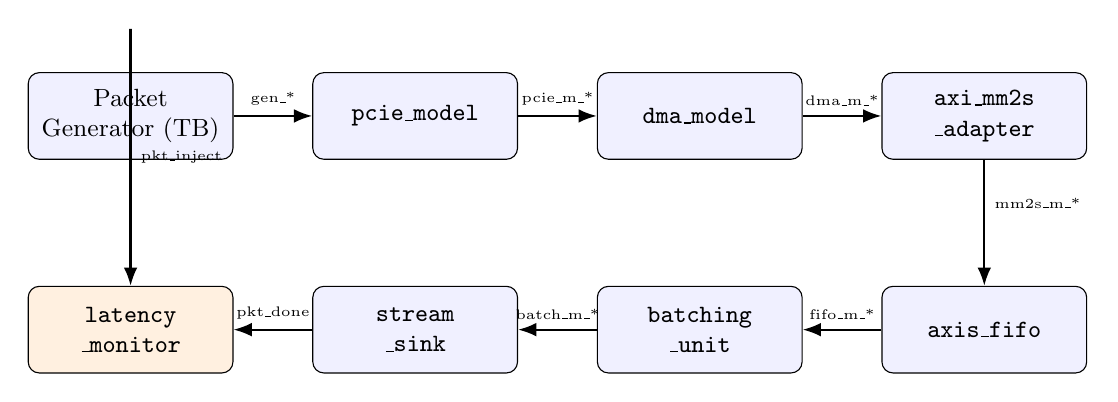
\begin{tikzpicture}[
  block/.style={draw, rounded corners, rectangle, minimum width=2.6cm, minimum height=1.1cm, align=center, font=\small, fill=blue!6},
  monblock/.style={draw, rounded corners, rectangle, minimum width=2.6cm, minimum height=1.1cm, align=center, font=\small, fill=orange!12},
  arrow/.style={-Latex, thick}
]
  \node[block] (gen)   {Packet\\Generator (TB)};
  \node[block, right=1.0cm of gen]  (pcie)  {\texttt{pcie\_model}};
  \node[block, right=1.0cm of pcie] (dma)   {\texttt{dma\_model}};
  \node[block, right=1.0cm of dma]  (mm2s)  {\texttt{axi\_mm2s}\\\texttt{\_adapter}};

  \node[block, below=1.6cm of mm2s]  (fifo)  {\texttt{axis\_fifo}};
  \node[block, left=1.0cm of fifo]   (batch) {\texttt{batching}\\\texttt{\_unit}};
  \node[block, left=1.0cm of batch]  (sink)  {\texttt{stream}\\\texttt{\_sink}};
  \node[monblock, left=1.0cm of sink] (mon)   {\texttt{latency}\\\texttt{\_monitor}};

  \draw[arrow] (gen)  -- node[above,font=\tiny]{gen\_*} (pcie);
  \draw[arrow] (pcie) -- node[above,font=\tiny]{pcie\_m\_*} (dma);
  \draw[arrow] (dma)  -- node[above,font=\tiny]{dma\_m\_*} (mm2s);
  \draw[arrow] (mm2s.south) -- ++(0,-0.55) -| node[pos=0.25,right,font=\tiny]{mm2s\_m\_*} (fifo.north);
  \draw[arrow] (fifo)  -- node[above,font=\tiny]{fifo\_m\_*} (batch);
  \draw[arrow] (batch) -- node[above,font=\tiny]{batch\_m\_*} (sink);
  \draw[arrow] (sink)  -- node[above,font=\tiny]{pkt\_done}   (mon);
  \draw[arrow] (gen.north) -- ++(0,0.55) -| node[pos=0.75,right,font=\tiny]{pkt\_inject} (mon.north);
\end{tikzpicture}
\caption{Pipeline architecture of the PCIe-AXI DMA streaming model. Solid arrows carry AXI4-Stream beats (\texttt{tvalid/tready/tdata/tkeep/tlast/tuser/tid}); the top-to-bottom arrow into \texttt{latency\_monitor} carries only the two scalar injection/completion event signals, not the data stream itself.}
\label{fig:pipeline_overview}
\end{figure}

Every solid arrow in \autoref{fig:pipeline_overview} is a full AXI4-Stream connection (Section~\ref{sec:ch3_axi}): \texttt{tvalid}, \texttt{tready}, \texttt{tdata}, \texttt{tkeep}, \texttt{tlast}, \texttt{tuser}, and \texttt{tid}. Because every stage implements its own independent \texttt{tvalid}/\texttt{tready} handshake, back-pressure asserted anywhere downstream (for example, a full FIFO) propagates correctly upstream through every intervening stage without any stage needing to know about the others -- a direct consequence of the AXI4-Stream composability property noted in \autoref{sec:ch3_axi}.

%----------------------------------------------------------------------------------------

\subsection{Shared Package and Sideband Signalling Convention}
\label{sec:ch4_sideband}

All modules and the testbench import a single SystemVerilog package, \texttt{pcie\_axi\_pkg}, which centralises every width and timing parameter (data width, packet-size field width, PCIe and DMA timing constants, FIFO depth, batch size, and so on) so that a single edit propagates consistently to every stage and to the sweep experiments of \autoref{Chapter7}. \autoref{tab:pkg_params} lists the default parameter values used throughout this thesis unless a specific experiment overrides them.

\begin{table}[htbp]
\centering
\begin{tabular}{@{}llrl@{}}
\toprule
\textbf{Parameter} & \textbf{Meaning} & \textbf{Default} & \textbf{Unit} \\
\midrule
\texttt{DATA\_WIDTH}        & AXI-Stream data bus width         & 64  & bits (8 B/beat) \\
\texttt{PKT\_SIZE\_W}       & Width of the packet-size field     & 13  & bits (0--8191 B) \\
\texttt{PKT\_ID\_W}         & Width of the packet tag field       & 8   & bits (0--255) \\
\texttt{PCIE\_BASE\_LATENCY}   & PCIe fixed per-TLP overhead      & 20  & cycles \\
\texttt{PCIE\_PER\_DW\_LATENCY}& PCIe per-DWORD overhead          & 1   & cycles/DWORD \\
\texttt{DMA\_SETUP\_CYCLES}    & DMA descriptor-fetch overhead    & 8   & cycles \\
\texttt{DMA\_BYTES\_PER\_CYC}  & DMA effective transfer rate      & 8   & bytes/cycle \\
\texttt{FIFO\_DEPTH\_DEFAULT}  & AXI-Stream FIFO depth            & 64  & beats \\
\texttt{BATCH\_COUNT\_DEFAULT} & Packets coalesced per batch      & 4   & packets \\
\texttt{BATCH\_TIMEOUT\_DEFAULT}& Idle cycles before forced flush & 64  & cycles \\
\bottomrule
\end{tabular}
\caption{Default parameters exported by \texttt{pcie\_axi\_pkg} and used throughout this thesis unless stated otherwise.}
\label{tab:pkg_params}
\end{table}

Two AXI4-Stream sideband fields are given a fixed, pipeline-wide meaning so that every stage, and the latency monitor, can recover per-packet metadata without a dedicated side channel:
\begin{itemize}
    \item \texttt{tuser} carries the packet's byte length (constant across every beat of a packet), which every stage that needs to compute a size-dependent delay (\texttt{pcie\_model}, \texttt{dma\_model}) or a size-dependent \texttt{tkeep} mask (\texttt{axi\_mm2s\_adapter}) reads directly rather than recomputing from a beat count.
    \item \texttt{tid} carries the packet's identifying tag, which the latency monitor uses to correlate an injection event with its corresponding completion event, since packets may in general be in flight and out of order with respect to other tagged events.
\end{itemize}

%----------------------------------------------------------------------------------------

\section{\texttt{pcie\_model}: PCIe Transaction-Layer Model}
\label{sec:ch4_pcie_model}

\texttt{pcie\_model} implements Equation~\ref{eq:pcie_latency} as a three-state finite-state machine (receive, delay, send). It buffers an entire incoming packet, computes its PCIe delay from the latched packet size once the packet's final beat (\texttt{tlast}) is seen, holds the packet for exactly that many cycles while de-asserting \texttt{s\_tready} (back-pressuring the packet generator), and then replays the buffered beats to \texttt{dma\_model}. Because the delay is computed once per packet from the packet's total size rather than per beat, this module reproduces the fixed-plus-proportional PCIe cost of \autoref{sec:ch3_pcie} exactly, including the tighter case of the module's internal buffer having to hold up to a full 4~KB packet (512 beats at the default 64-bit bus width). The detailed state-transition behaviour is presented in \autoref{sec:ch5_pcie_fsm}.

\section{\texttt{dma\_model}: DMA Engine Model}
\label{sec:ch4_dma_model}

\texttt{dma\_model} implements Equation~\ref{eq:dma_latency} with an analogous three-state structure (receive, setup, send). After buffering a full packet from \texttt{pcie\_model}, it spends a fixed \texttt{SETUP\_CYCLES} modelling descriptor fetch and doorbell processing (\autoref{sec:ch3_dma}), and then plays the packet out at a rate governed by \texttt{DMA\_BYTES\_PER\_CYC}: at the default rate (equal to the bus width), one beat is produced per cycle with no throttling; at a reduced rate, an inter-beat holdoff models a bandwidth-limited memory read. This throttle exists so the model can, if required, separate DMA-side bandwidth limitations from the fixed setup overhead that is the focus of this thesis. \autoref{sec:ch5_dma_fsm} gives the full state-transition detail.

\section{\texttt{axi\_mm2s\_adapter}: Memory-Mapped-to-Stream Adapter}
\label{sec:ch4_mm2s}

\texttt{axi\_mm2s\_adapter} models the final re-packetisation stage of a real \ac{MM2S} DMA path, in which pre-staged payload bytes are serialised onto an AXI4-Stream bus. Because this thesis's upstream stages already deliver data beat-by-beat, the adapter's only substantive function is combinational: it computes the correct \texttt{tkeep} mask for the final beat of every packet, using the packet's byte length (via \texttt{tuser}) modulo the bus width in bytes, so that a packet whose length is not an exact multiple of the bus width correctly marks only its valid trailing bytes. The adapter adds no pipeline stages and hence no latency of its own -- architecturally correct, since in a real system this logic is folded into the DMA engine itself rather than existing as a separate, registered stage.

\section{\texttt{axis\_fifo}: Parameterised AXI-Stream FIFO}
\label{sec:ch4_fifo}

\texttt{axis\_fifo} is a synchronous, first-word-fall-through (\ac{FWFT}) circular buffer of configurable depth \texttt{DEPTH}, decoupling the (potentially bursty) production rate of the upstream DMA path from the consumption rate of whatever sits downstream. Because its read side is combinational (the head-of-queue entry is presented on \texttt{m\_tdata} as soon as the FIFO is non-empty, with no extra registered pull stage), the FIFO adds zero cycles of latency to a packet that finds it empty on arrival -- latency only appears once the write side stalls because the FIFO is full. This property is what makes the FIFO-depth experiment of \autoref{sec:ch7_fifo_stall} meaningful only under a rate-limited consumer: with an always-ready sink, the FIFO drains every cycle it holds data and can never accumulate occupancy, so depth has no observable effect (\autoref{sec:ch7_fifo_always_ready}). The module also exposes an \texttt{occupancy} output and \texttt{full}/\texttt{empty} flags used directly by the testbench's FIFO-stress instrumentation (\autoref{sec:ch6_testbench}).

\section{\texttt{batching\_unit}: Small-Packet Batching Unit}
\label{sec:ch4_batching_unit}

\texttt{batching\_unit} is the RTL realisation of the overhead-amortisation principle motivated in \autoref{sec:ch2_batching} and formalised in Equation~\ref{eq:batch_inequality}. It is an online, zero-buffering pass-through stage: every beat flows from its slave port to its master port on the same cycle, and the unit modifies only the packet-boundary signalling, not the data itself. While counting inner packets, it suppresses every \texttt{tlast} that would otherwise mark the end of an individual small packet, and instead asserts a single \texttt{tlast} once either \texttt{BATCH\_COUNT} packets have been accumulated or an idle-cycle timeout (\texttt{BATCH\_TIMEOUT}) forces an early flush. The resulting single, larger frame carries the accumulated total byte count on \texttt{tuser} and the tag of its first constituent packet on \texttt{tid}, so that downstream stages -- in particular the latency monitor -- correctly attribute the whole coalesced frame to one measurement rather than to its first inner packet's original size. When disabled (\texttt{enable=0}), the unit degenerates to a zero-latency combinational pass-through, which is what makes the un-batched baseline of \autoref{Chapter7} a fair, single-parameter A/B comparison against the batched configuration. The full batching algorithm and its corner cases are detailed in \autoref{sec:ch5_batching}.

\section{\texttt{stream\_sink}: Terminal Consumer and Completion Signalling}
\label{sec:ch4_stream_sink}

\texttt{stream\_sink} represents the endpoint consumer of the pipeline -- conceptually, a PCIe device receive buffer, a network MAC, or a host-side write target. By default it is permanently ready (\texttt{s\_tready = 1}), so that the datapath's measured latency reflects only the PCIe/DMA/buffering path and is not confounded by consumer-side back-pressure; an optional configurable stall model (accepting only a fraction of cycles, parameterised by \texttt{STALL\_PERIOD}/\texttt{STALL\_READY}) is provided specifically to exercise the FIFO-depth experiment of \autoref{sec:ch7_fifo_stall}, since an always-ready sink never allows the upstream FIFO to accumulate occupancy. On every beat that is both valid and accepted with \texttt{tlast} asserted, the sink emits a one-cycle \texttt{pkt\_done} pulse together with the completing packet's tag (\texttt{done\_id}) and its actual byte count (\texttt{done\_size}, batch-aware -- i.e. the total frame size when the batching unit is active) to the latency monitor.

\section{\texttt{latency\_monitor}: Hardware Latency Measurement}
\label{sec:ch4_latency_monitor}

\texttt{latency\_monitor} is a hardware performance-counter block, not a testbench artefact: it is instantiated inside the design itself and measures latency using only signals available in hardware. It maintains a free-running cycle counter and, indexed by packet tag, a table of injection timestamps and injected sizes. When a \texttt{pkt\_inject} event arrives (asserted by the packet generator at the same cycle the first beat of a packet is presented), the current cycle count and size are recorded against that packet's tag; when the corresponding \texttt{pkt\_done} event arrives from \texttt{stream\_sink}, the elapsed cycle count since injection is computed and registered as that packet's latency, together with running minimum, maximum, average, and throughput statistics reported at the end of simulation. Because injection and completion are both hardware events on the same clock domain, this measurement is immune to the kind of software-side reference-point misalignment that produced a spurious constant offset in an earlier iteration of the testbench (\autoref{sec:ch6_milestones}), and its output is what is reported directly as the \texttt{[RESULT]} rows analysed in \autoref{Chapter7}.

%----------------------------------------------------------------------------------------

\section{Top-Level Integration and Parameterisation}
\label{sec:ch4_top}

\texttt{pcie\_axi\_dma\_top} instantiates and wires together the seven stages of \autoref{fig:pipeline_overview} using a consistent per-stage AXI4-Stream bus naming convention (\texttt{<stage>\_tvalid}, \texttt{<stage>\_tready}, and so on), and re-exports, as module parameters, every configuration knob needed to run the experiments of \autoref{Chapter7} without editing RTL: the PCIe and DMA timing constants, the FIFO depth, the batch count and timeout, a single \texttt{BATCHING\_EN} bit that switches the batching unit between bypass and active modes, and the stream-sink stall parameters. Exposing \texttt{BATCHING\_EN} as a synthesis-time parameter rather than a runtime signal was a deliberate choice: it allows a downstream synthesis tool to prune the entire batching datapath in the baseline configuration, and it guarantees that the baseline and batched configurations of \autoref{sec:ch7_batching} differ in exactly one bit at elaboration time, isolating the effect being measured.
 
% Chapter 5

\chapter{Design and Implementation}

\label{Chapter5}

\lhead{Chapter 5. \emph{Design and Implementation}}

This chapter details the design methodology followed while implementing the architecture of \autoref{Chapter4}, the finite-state-machine designs of the two timing-critical stages (\texttt{pcie\_model} and \texttt{dma\_model}), the packet-batching algorithm, and the implementation of the hardware latency monitor, including a timing subtlety that was discovered and corrected during development.

%----------------------------------------------------------------------------------------

\section{Design Methodology}
\label{sec:ch5_methodology}

The pipeline was built incrementally, one stage at a time, rather than as a single monolithic design, for two reasons specific to a latency-measurement study. First, because every stage communicates with its neighbours purely through the AXI4-Stream handshake of \autoref{sec:ch3_axi}, each stage could be developed and elaborated against stub (safe-default-output) versions of the stages not yet implemented, so the design always elaborated and simulated to completion, giving a continuously green baseline to build on. Second, because the object of study is \emph{where} latency is spent, each stage's timing contribution needed to be independently attributable; building and testing \texttt{pcie\_model} in isolation before adding \texttt{dma\_model}, for example, made it possible to confirm each stage's measured delay against Equations~\ref{eq:pcie_latency}--\ref{eq:dma_latency} before composing it with the next stage, rather than debugging an aggregate number that could hide a compensating pair of errors.

All modules follow the same coding conventions: parameters default to values imported from the shared \texttt{pcie\_axi\_pkg} package (\autoref{tab:pkg_params}) but can be overridden per instantiation; sequential logic is written with \texttt{always\_ff} blocks synchronous to \texttt{clk} with asynchronous active-low reset; and all diagnostic \texttt{\$display}/\texttt{\$warning} statements are wrapped in \texttt{synthesis translate\_off}/\texttt{translate\_on} pairs so the modules remain synthesisable despite the simulation-only instrumentation used for the results of \autoref{Chapter7}.

%----------------------------------------------------------------------------------------

\section{\texttt{pcie\_model} Finite-State-Machine Design}
\label{sec:ch5_pcie_fsm}

\autoref{fig:pcie_fsm} shows the three-state machine that implements the PCIe transaction-layer delay of Equation~\ref{eq:pcie_latency}.

\begin{figure}[htbp]
\centering
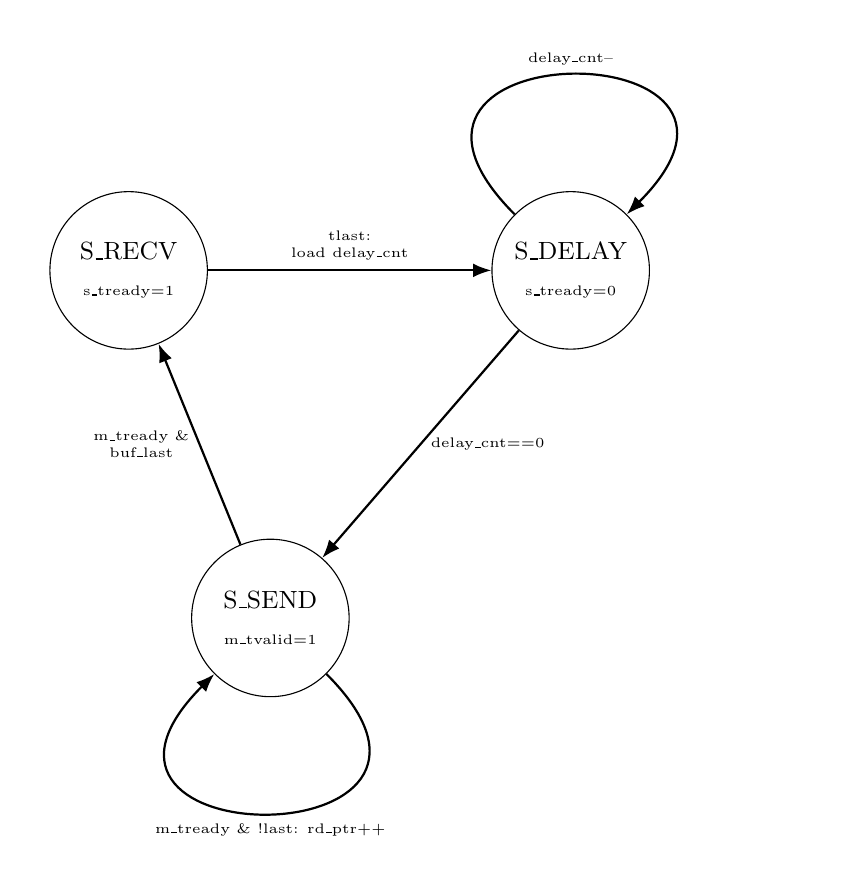
\begin{tikzpicture}[
  state/.style={draw, circle, minimum size=2.0cm, align=center, font=\small},
  arrow/.style={-Latex, thick}
]
  \node[state] (recv)  {S\_RECV\\[2pt]{\tiny s\_tready=1}};
  \node[state, right=3.6cm of recv] (delay) {S\_DELAY\\[2pt]{\tiny s\_tready=0}};
  \node[state, below=2.4cm of recv, xshift=1.8cm] (send)  {S\_SEND\\[2pt]{\tiny m\_tvalid=1}};

  \draw[arrow] (recv) -- node[above,font=\tiny,align=center]{tlast:\\load delay\_cnt} (delay);
  \draw[arrow] (delay) -- node[right,font=\tiny,align=center]{delay\_cnt==0} (send);
  \draw[arrow] (send) -- node[left,font=\tiny,align=center]{m\_tready \&\\buf\_last} (recv);
  \draw[arrow] (delay) to[out=135,in=45,looseness=6] node[above,font=\tiny]{delay\_cnt--} (delay);
  \draw[arrow] (send) to[out=-45,in=-135,looseness=6] node[below,font=\tiny]{m\_tready \& !last: rd\_ptr++} (send);
\end{tikzpicture}
\caption{\texttt{pcie\_model} state machine. The packet is fully buffered in S\_RECV, held for \texttt{computed\_delay} $= T_{base} + \lceil S/4\rceil \cdot T_{dw}$ cycles in S\_DELAY, then replayed beat-by-beat in S\_SEND.}
\label{fig:pcie_fsm}
\end{figure}

In \textbf{S\_RECV}, \texttt{s\_tready} is asserted and every incoming beat is written into an internal packet buffer sized for the largest packet under test (4~KB, i.e.\ 512 beats at the default 64-bit bus width); when \texttt{s\_tlast} is seen, the per-packet size and tag are latched from \texttt{tuser}/\texttt{tid}, the delay counter is loaded combinationally from \texttt{computed\_delay = BASE\_LATENCY + ((pkt\_size+3)>>2) * PER\_DW\_LATENCY} (an integer formulation of $\lceil S/4\rceil$ that avoids a division operator), and the machine moves to \textbf{S\_DELAY}. In S\_DELAY, \texttt{s\_tready} is de-asserted -- back-pressuring the packet generator for the duration of the modelled PCIe delay -- and the counter is decremented once per cycle until it reaches zero, at which point the machine moves to \textbf{S\_SEND} and begins driving the buffered beats to \texttt{dma\_model}, honouring \texttt{m\_tready} back-pressure and returning to S\_RECV once the buffered \texttt{tlast} beat is accepted. Because exactly one packet is buffered and replayed at a time (matching the sequential, one-packet-in-flight injection pattern of the testbench described in \autoref{sec:ch6_testbench}), the buffer indexing requires no wrap-around logic beyond a simple reset-to-zero on each packet boundary.

%----------------------------------------------------------------------------------------

\section{\texttt{dma\_model} Finite-State-Machine Design}
\label{sec:ch5_dma_fsm}

\autoref{fig:dma_fsm} shows the analogous three-state machine implementing the DMA descriptor-processing delay of Equation~\ref{eq:dma_latency}.

\begin{figure}[htbp]
\centering
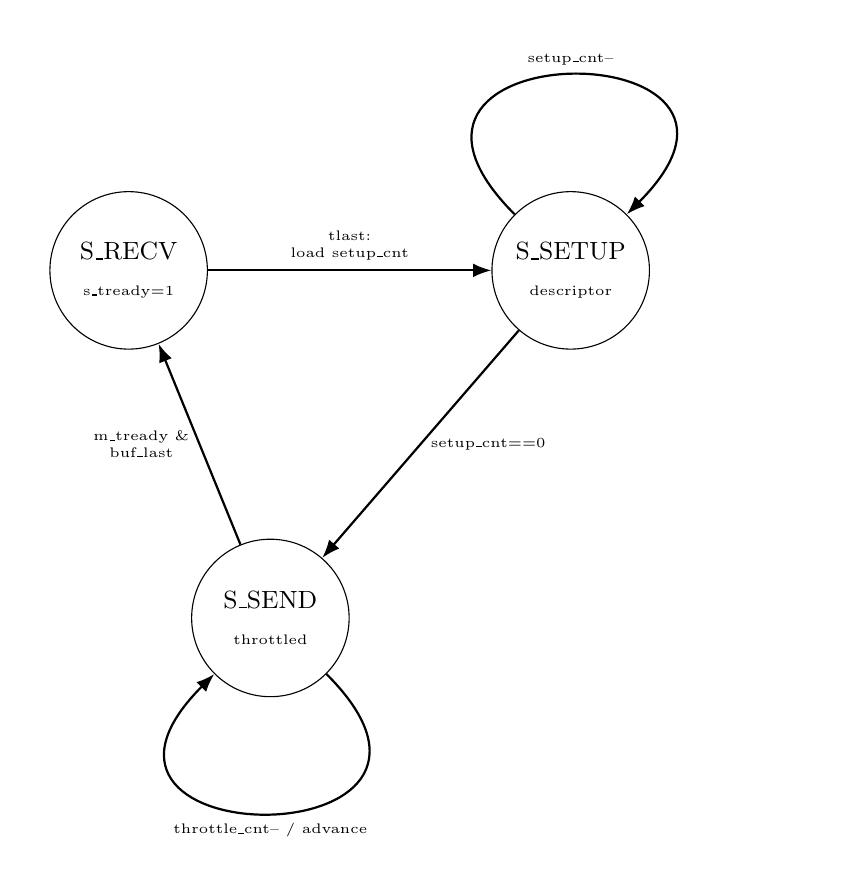
\begin{tikzpicture}[
  state/.style={draw, circle, minimum size=2.0cm, align=center, font=\small},
  arrow/.style={-Latex, thick}
]
  \node[state] (recv)   {S\_RECV\\[2pt]{\tiny s\_tready=1}};
  \node[state, right=3.6cm of recv]  (setup)  {S\_SETUP\\[2pt]{\tiny descriptor}};
  \node[state, below=2.4cm of recv, xshift=1.8cm] (send)   {S\_SEND\\[2pt]{\tiny throttled}};

  \draw[arrow] (recv) -- node[above,font=\tiny,align=center]{tlast:\\load setup\_cnt} (setup);
  \draw[arrow] (setup) -- node[right,font=\tiny,align=center]{setup\_cnt==0} (send);
  \draw[arrow] (send) -- node[left,font=\tiny,align=center]{m\_tready \&\\buf\_last} (recv);
  \draw[arrow] (setup) to[out=135,in=45,looseness=6] node[above,font=\tiny]{setup\_cnt--} (setup);
  \draw[arrow] (send) to[out=-45,in=-135,looseness=6] node[below,font=\tiny]{throttle\_cnt-- / advance} (send);
\end{tikzpicture}
\caption{\texttt{dma\_model} state machine. S\_SETUP models the fixed \texttt{SETUP\_CYCLES} descriptor-fetch overhead of Section~\ref{sec:ch3_dma}; S\_SEND plays out beats at a rate set by \texttt{BYTES\_PER\_CYC}, with an inter-beat holdoff (\texttt{throttle\_cnt}) only when the modelled DMA rate is below the bus's native rate.}
\label{fig:dma_fsm}
\end{figure}

The behaviour mirrors \texttt{pcie\_model} with one addition: in \textbf{S\_SEND}, a \texttt{throttle\_cnt} counter models a DMA engine reading from memory slower than the AXI-Stream bus's native rate. \texttt{CYCLES\_PER\_BEAT} is derived at elaboration time as $\lceil W_{bus} / \text{BYTES\_PER\_CYC} \rceil$, where $W_{bus}$ is the bus width in bytes; at the default configuration (\texttt{BYTES\_PER\_CYC} equal to the bus width), \texttt{CYCLES\_PER\_BEAT = 1} and every beat is produced with no holdoff, so the transfer-phase contribution to Equation~\ref{eq:dma_latency} reduces exactly to the number of beats in the packet. A reduced \texttt{BYTES\_PER\_CYC} (e.g.\ modelling a slower DRAM back-end) inserts a proportional holdoff between beats, which is available as an experimental knob but is held at its full-rate default throughout the results of \autoref{Chapter7}, since this thesis's focus is the fixed setup term rather than DMA-side memory bandwidth.

Both FSMs report their key internal timing events via simulation-only \texttt{\$display} statements -- \texttt{pcie\_model} warns if its buffer nears the size limit set by the 4~KB test packet, and \texttt{dma\_model} reports the exact cycle at which each packet's descriptor-setup countdown completes -- which were used during development to cross-check each stage's contribution against Equations~\ref{eq:pcie_latency}--\ref{eq:dma_latency} before the stages were composed together.

%----------------------------------------------------------------------------------------

\section{Small-Packet Batching Algorithm}
\label{sec:ch5_batching}

The batching unit (\autoref{sec:ch4_batching_unit}) is implemented as an online pass-through with a small amount of counting state rather than a buffering stage, so that it adds no latency of its own beyond the coalescing effect it is designed to produce. \autoref{alg:batching} summarises its per-beat decision logic.

\begin{table}[htbp]
\centering
\begin{tabular}{@{}p{0.95\textwidth}@{}}
\toprule
\textbf{Algorithm: per-beat batching decision} (executed every cycle a beat is accepted, i.e.\ \texttt{s\_tvalid \&\& m\_tready}) \\
\midrule
1. Pass \texttt{tdata}/\texttt{tkeep} through unchanged (zero-latency wiring). \\
2. If this is the first beat of a new batch, latch \texttt{first\_id} $\leftarrow$ \texttt{s\_tid}. \\
3. If \texttt{s\_tlast} is asserted (an inner packet boundary): \\
\quad a. Accumulate \texttt{pkt\_cnt} $\leftarrow$ \texttt{pkt\_cnt} + 1 and \texttt{batch\_bytes} $\leftarrow$ \texttt{batch\_bytes} + \texttt{s\_tuser}. \\
\quad b. If \texttt{pkt\_cnt} has now reached \texttt{BATCH\_COUNT}, or a timeout flush is pending: assert \texttt{m\_tlast}, drive \texttt{m\_tuser} = accumulated \texttt{batch\_bytes}, drive \texttt{m\_tid} = \texttt{first\_id}, and reset all batch state. \\
\quad c. Otherwise, suppress \texttt{m\_tlast} (the inner boundary is invisible downstream) and continue accumulating. \\
4. If no beat is accepted for \texttt{BATCH\_TIMEOUT} consecutive cycles while a batch is in progress, set \texttt{flush\_pending}, causing the \emph{next} \texttt{tlast} to close the batch regardless of \texttt{pkt\_cnt} (prevents an indefinite hang on a short final batch). \\
\bottomrule
\end{tabular}
\caption{Batching-unit decision logic executed on every accepted beat.}
\label{alg:batching}
\end{table}

Two design details are worth making explicit. First, \texttt{m\_tuser} is only architecturally meaningful at the beat where \texttt{m\_tlast} is asserted (the only beat \texttt{stream\_sink} actually reads it on), so the running partial sum on intermediate beats is a "don't care" for correctness -- this simplifies the combinational output mux at the cost of a value that would be misleading if inspected mid-batch. Second, the module is parameterised by a single \texttt{enable} input, and when \texttt{enable=0} every output is wired directly from the corresponding input with no counting logic in the path at all; this is what allows the baseline (\autoref{sec:ch7_baseline}) and batched (\autoref{sec:ch7_batching}) configurations to be produced from the same RTL and the same testbench, differing only in this one bit, giving a clean, controlled A/B comparison rather than two independently-built designs that might differ in unintended ways.

The corner case noted in \autoref{sec:ch4_batching_unit} -- an incomplete final batch with no further \texttt{tlast} to trigger the timeout flush -- was a deliberate scope decision: the testbench's batching scenario (\autoref{sec:ch6_testbench}) always injects exactly \texttt{BATCH\_COUNT} packets, so the corner case does not arise in any experiment reported in this thesis, but it is recorded here as a known limitation of the current implementation (revisited in \autoref{sec:ch8_limitations}).

%----------------------------------------------------------------------------------------

\section{Hardware Latency Monitor: Implementation and a Timing Correction}
\label{sec:ch5_latmon_impl}

The latency monitor's core measurement is a subtraction between two cycle-counter samples: an injection timestamp, recorded when \texttt{pkt\_inject} fires, and a completion timestamp, recorded when the corresponding \texttt{pkt\_done} fires. Both events are registered, one-cycle pulses, and the free-running \texttt{cycle\_cnt} they are compared against is read by both always-block instances in the same active region, so the computed difference is an exact integer number of clock periods between the two hardware events, with no possibility of an off-by-one error from mixing pre- and post-edge values.

An earlier iteration of the testbench, however, computed a second, independent latency figure in software using its own local cycle counter, sampled one cycle \emph{before} the point at which the corresponding hardware event actually registered. This produced a constant, systematic two-cycle discrepancy between the testbench's self-reported latency and the hardware latency monitor's figure -- consistent across every packet size, and hence a fixed measurement-methodology artefact rather than a functional bug in the pipeline itself. The fix, described further in \autoref{sec:ch6_milestones}, was to make the testbench's reported \texttt{[RESULT]} rows read \texttt{latency\_out} directly from the hardware monitor rather than recomputing it independently, which by construction eliminates any possibility of the two figures disagreeing. This episode is recorded here because it illustrates a general methodological point relevant to any latency study of this kind: once both a device-under-test-side measurement and a testbench-side measurement exist, they must be reconciled to a single reference point, or an artefact of the measurement apparatus can be mistaken for a property of the design under test.

A second, batching-specific detail in the monitor's implementation is worth noting. \texttt{size\_store[id]}, populated at injection time, records the size of the individual packet that was injected, while \texttt{done\_size}, supplied by \texttt{stream\_sink} at completion time, records the actual size of whatever frame closed -- the full batch total when the batching unit is active. The monitor's efficiency and throughput statistics are computed from \texttt{done\_size}, not \texttt{size\_store}, specifically so that a coalesced batch is correctly reported at its true aggregate size rather than at the size of only its first constituent packet; the breakdown estimator (the per-packet \texttt{est:} diagnostic line) additionally compares these two values to detect whether a given completion is a single packet or a batch, and selects the appropriate closed-form latency estimate (Equation~\ref{eq:total_latency} for a single packet, or its $N$-fold serial extension implied by Equation~\ref{eq:batch_inequality} for a batch) accordingly.
 
% Chapter 6

\chapter{Experimental Setup and Work Completed}

\label{Chapter6}

\lhead{Chapter 6. \emph{Experimental Setup and Work Completed}}

This chapter describes the simulation environment used to exercise the architecture of \autoref{Chapter4}, the testbench that drives and measures it, and a chronological account of the verification milestones -- including two measurement-methodology bugs discovered and fixed during development -- that led to the results reported in \autoref{Chapter7}.

%----------------------------------------------------------------------------------------

\section{Simulation Environment}
\label{sec:ch6_simenv}

All RTL is compiled, elaborated, and simulated with the AMD-Xilinx Vivado \texttt{xsim} logic simulator \cite{xilinx2022vivadosim}, driven through a project \texttt{Makefile} rather than the Vivado GUI, so that every configuration used in this thesis is reproducible from a single command line. The flow has three stages, matching the standard \texttt{xsim} toolchain:

\begin{enumerate}
    \item \textbf{Compile} (\texttt{xvlog --sv}) -- all nine SystemVerilog sources (\texttt{pcie\_axi\_pkg.sv} through \texttt{pcie\_axi\_dma\_top.sv}, plus the testbench) are compiled incrementally into a shared work library.
    \item \textbf{Elaborate} (\texttt{xelab}) -- the testbench top-level is elaborated into a named snapshot, with every scenario/configuration parameter (\autoref{sec:ch6_testbench}) passed as a \texttt{-generic\_top} override so that no RTL edit is required to change a run's configuration.
    \item \textbf{Simulate} (\texttt{xsim ---runall}) -- the snapshot is run to completion in batch mode (or, for waveform debugging, under the \texttt{xsim} GUI with a saved waveform database).
    \end{enumerate}

The \texttt{Makefile} tracks compilation and elaboration with file-timestamp sentinels, and additionally fingerprints the exact generics string used for the previous elaboration; this second check exists because \texttt{xelab}'s snapshot is otherwise silently reused across a plain \texttt{make sim} invocation with different generics, which would cause a scenario or parameter sweep to report stale results from the previous configuration without any warning. Targets are provided for a single run (\texttt{make sim TB\_SCENARIO=\ldots}), a FIFO-depth sweep under an always-ready sink (\texttt{make fifo-sweep}), the same sweep under a rate-limited sink (\texttt{make fifo-sweep-stall}), and a full regression that executes every scenario used in this thesis and collects all \texttt{[RESULT]} rows into a single log (\texttt{make sim-all}).

%----------------------------------------------------------------------------------------

\section{Testbench Architecture}
\label{sec:ch6_testbench}

The testbench, \texttt{tb\_pcie\_axi\_dma}, instantiates \texttt{pcie\_axi\_dma\_top} (\autoref{sec:ch4_top}), generates a 100~MHz clock, and drives one of three scenarios selected by the \texttt{TB\_SCENARIO} parameter, summarised in \autoref{tab:tb_scenarios}.

\begin{table}[htbp]
\centering
\begin{tabular}{@{}clp{7.2cm}@{}}
\toprule
\textbf{TB\_SCENARIO} & \textbf{Name} & \textbf{Description} \\
\midrule
0 & Baseline    & Batching disabled; one packet of each of six sizes (64~B, 128~B, 256~B, 512~B, 1~KB, 4~KB) is injected in turn and its latency measured (\autoref{sec:ch7_baseline}). \\
1 & Batching    & Batching enabled; \texttt{BATCH\_COUNT} (default 4) $\times$ 64~B packets are injected back-to-back and the latency of the single resulting coalesced frame is measured (\autoref{sec:ch7_batching}). \\
2 & FIFO sweep  & Batching disabled, identical to Scenario~0's packet-size loop, but intended to be re-run at \texttt{FIFO\_DEPTH} $\in \{16, 64, 256\}$, optionally with the sink stall model enabled, to study buffering behaviour (\autoref{sec:ch7_fifo}). \\
\bottomrule
\end{tabular}
\caption{Testbench scenarios selected via the \texttt{TB\_SCENARIO} elaboration-time parameter.}
\label{tab:tb_scenarios}
\end{table}

For Scenarios 0 and 2, the main test loop drives each packet size in turn via a \texttt{send\_packet} task, waits for the pipeline's \texttt{pkt\_count} output to increment (indicating \texttt{stream\_sink} has accepted that packet's final beat), waits one further clock edge for the hardware latency monitor to register \texttt{latency\_out} (\autoref{sec:ch4_latency_monitor}), and then prints a \texttt{[RESULT]} row giving the packet ID, size, measured latency, computed efficiency (Equation~\ref{eq:efficiency}), the peak FIFO occupancy observed during that packet's transit, and whether the FIFO was ever observed full. Scenario~1 differs only in that it injects \texttt{BATCH\_COUNT} packets before waiting for a single completion event, since the batching unit (\autoref{sec:ch5_batching}) coalesces them into one frame. A global watchdog (a plain \texttt{initial} block with a fixed time limit) terminates the simulation and reports an error if any packet fails to complete within a generous margin of its worst-case expected latency, so a regression run cannot hang silently.

\subsection{The \texttt{send\_packet} Handshake and Its Correction}
\label{sec:ch6_send_packet}

The \texttt{send\_packet} task drives every beat of one packet's \texttt{gen\_*} inputs and must correctly detect, on the final beat, that \texttt{pcie\_model} (\autoref{sec:ch5_pcie_fsm}) has accepted it before de-asserting \texttt{gen\_tvalid}. The subtlety is that \texttt{pcie\_model}'s \texttt{s\_tready} is combinationally derived from its current state (\texttt{state == S\_RECV}), and that state only transitions to \texttt{S\_DELAY} \emph{after} the active simulation region in which the final beat's acceptance is decided. An earlier version of this task polled \texttt{gen\_tready} using \texttt{while (!gen\_tready) @(posedge clk);}, which sampled \texttt{gen\_tready} \emph{after} the non-blocking state update had already taken effect for that edge and therefore observed \texttt{s\_tready} having already dropped for the packet's own final beat, causing the task to hang waiting for an acceptance that had, in fact, already occurred. The fix -- checking \texttt{gen\_tready} inside a \texttt{do \ldots\ @(posedge clk); end while} construct, so the check happens in the active (pre-non-blocking-assignment) region for every beat, including the last -- resolved this and is the form of the task used for every result reported in this thesis.

%----------------------------------------------------------------------------------------

\section{Verification Milestones and Bugs Found}
\label{sec:ch6_milestones}

The pipeline was brought up and verified incrementally, stage by stage, following the design methodology of \autoref{sec:ch5_methodology}. \autoref{tab:milestones} summarises the sequence of milestones and the issues resolved at each stage.

\begin{table}[htbp]
\centering
\begin{tabular}{@{}p{2.6cm}p{9.7cm}@{}}
\toprule
\textbf{Milestone} & \textbf{Outcome} \\
\midrule
% Architecture \& stubs & Package, top-level wiring, and stub modules with safe default outputs elaborate and \texttt{\$finish} cleanly, giving a green baseline for incremental development. \\
% \texttt{pcie\_model} & Three-state FSM implemented and its computed delay cross-checked by hand against Equation~\ref{eq:pcie_latency} for all six test packet sizes. \\
\texttt{dma\_model} & Three-state FSM implemented; descriptor-setup overhead fraction computed for 64~B/512~B/4~KB packets (50\%, 11\%, and 1.5\% of total DMA-stage cycles respectively), directly motivating the batching experiment of \autoref{sec:ch7_batching}. \\
\texttt{axi\_mm2s}, \texttt{axis\_fifo} &
Zero-latency \texttt{tkeep} correction and FWFT FIFO, verified using hand-computed \texttt{tkeep} masks for unaligned packet sizes. \\
\texttt{stream\_sink} \& first end-to-end run & First complete pipeline run (bypass mode, \texttt{FIFO\_DEPTH=64}) produced a full latency/efficiency table across all six packet sizes; the \texttt{send\_packet} handshake bug of \autoref{sec:ch6_send_packet} was found and fixed at this stage, since it only manifests once a real multi-stage DUT can actually assert back-pressure on the last beat. \\
\texttt{latency\_monitor} & Hardware latency monitor added; its measurements agreed with the testbench's own figures to within a constant $\pm 2$ cycles, which was traced to the testbench sampling its reference point one cycle before the corresponding hardware event (\autoref{sec:ch5_latmon_impl}) and fixed by making \texttt{[RESULT]} rows read \texttt{latency\_out} directly. \\
\texttt{batching\_unit} & Batching FSM verified directly against its simulation diagnostics: three intermediate \texttt{tlast} pulses correctly suppressed, the fourth correctly closing the batch with the expected accumulated byte count and first-packet tag, and inter-packet gaps confirmed to remain below \texttt{BATCH\_TIMEOUT} so no spurious flush occurred. \\
Batch-mode efficiency bug & The latency monitor initially reported batch efficiency using each packet's \emph{individual} injected size (64~B) rather than the completed frame's true size (256~B), understating efficiency by $4\times$; fixed by routing \texttt{stream\_sink}'s batch-aware \texttt{done\_size} into the efficiency calculation instead of the per-injection \texttt{size\_store} table (\autoref{sec:ch5_latmon_impl}). \\
\texttt{stream\_sink} stall-model bug & Adding the optional consumer back-pressure model (needed for the FIFO-depth experiment of \autoref{sec:ch7_fifo_stall}) exposed a latent correctness bug: \texttt{pkt\_done} had been qualified only on \texttt{(s\_tvalid \&\& s\_tlast)}, which is a valid "beat transferred" check only when \texttt{s\_tready} is permanently 1. Under the stall model, \texttt{tvalid}/\texttt{tlast} can remain asserted for several cycles while waiting for \texttt{tready}, so the old check fired \texttt{pkt\_done} once per waiting cycle instead of once per actual transfer, quadrupling the reported \texttt{pkt\_count}. Fixed by correctly gating on \texttt{(s\_tvalid \&\& s\_tready \&\& s\_tlast)}. \\
\texttt{fifo\_occupancy} width bug & The top-level \texttt{fifo\_occupancy} output port was sized from the package default \texttt{FIFO\_DEPTH} (64) rather than the actual \texttt{FIFO\_DEPTH} parameter passed to that instance, silently truncating the reported occupancy for \texttt{FIFO\_DEPTH=256} runs. Fixed by sizing the port from \texttt{\$clog2(FIFO\_DEPTH)} using the instance's own parameter. \\
\bottomrule
\end{tabular}
\caption{Verification milestones completed during development, in chronological order, with the issues found and corrected at each stage.}
\label{tab:milestones}
\end{table}

By the end of this sequence, eight regression runs -- the baseline (Scenario~0), the batching experiment (Scenario~1), the FIFO-depth sweep at three depths under an always-ready sink, and the same sweep at three depths under the rate-limited stall model -- all completed without a simulation timeout, an assertion failure, or a watchdog firing, and are the runs analysed in \autoref{Chapter7}.
 
% Chapter 7

\chapter{Results and Analysis}

\label{Chapter7}

\lhead{Chapter 7. \emph{Results and Analysis}}

This chapter presents the simulation results obtained from the eight regression runs summarised in \autoref{tab:milestones}: the baseline packet-size sweep, the per-stage latency breakdown, the batching experiment, and the FIFO-depth sweep under both an always-ready and a rate-limited consumer. All latency figures are hardware-measured values read directly from \texttt{latency\_out} (\autoref{sec:ch4_latency_monitor}), not software-computed estimates, at a 100~MHz (10~ns period) simulation clock.

%----------------------------------------------------------------------------------------

\section{Baseline Latency and Efficiency versus Packet Size}
\label{sec:ch7_baseline}

\autoref{tab:baseline_results} reports the measured end-to-end latency and effective efficiency (Equation~\ref{eq:efficiency}) for the six packet sizes exercised by Scenario~0 (\autoref{tab:tb_scenarios}), with batching disabled and \texttt{FIFO\_DEPTH=64}.

\begin{table}[htbp]
\centering
\begin{tabular}{@{}rrr@{}}
\toprule
\textbf{Packet Size (B)} & \textbf{Latency (cycles)} & \textbf{Efficiency (B/cycle)} \\
\midrule
64    & 71   & 0.90 \\
128   & 111  & 1.15 \\
256   & 191  & 1.34 \\
512   & 351  & 1.46 \\
1024  & 671  & 1.53 \\
4096  & 2591 & 1.58 \\
\bottomrule
\end{tabular}
\caption{Baseline (un-batched) latency and efficiency versus packet size, \texttt{FIFO\_DEPTH=64}, always-ready sink.}
\label{tab:baseline_results}
\end{table}

\begin{figure}[htbp]
\centering
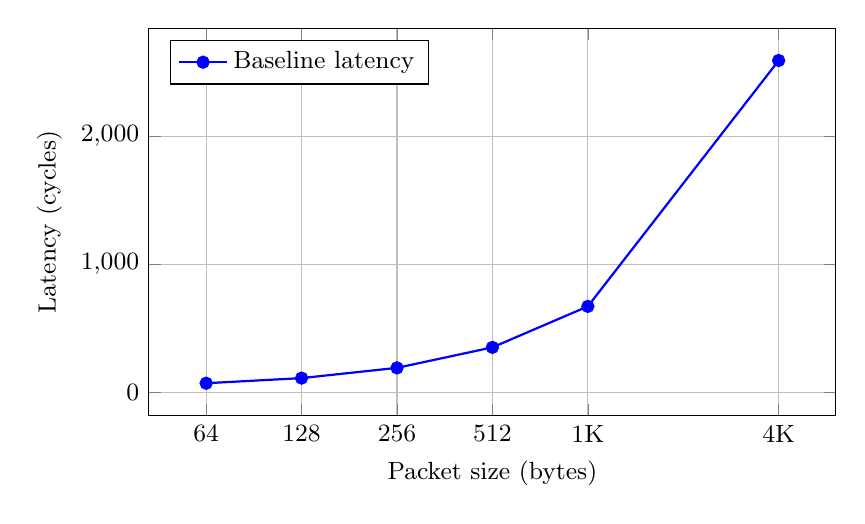
\begin{tikzpicture}
\begin{axis}[
    width=0.85\textwidth, height=6.5cm,
    xlabel={Packet size (bytes)}, ylabel={Latency (cycles)},
    xmode=log, log basis x=2,
    xtick={64,128,256,512,1024,4096},
    xticklabels={64,128,256,512,1K,4K},
    grid=major, legend pos=north west, font=\small
]
\addplot[mark=*, thick, blue] coordinates {(64,71) (128,111) (256,191) (512,351) (1024,671) (4096,2591)};
\legend{Baseline latency}
\end{axis}
\end{tikzpicture}
\caption{Measured baseline end-to-end latency versus packet size (log-scale x-axis).}
\label{fig:baseline_latency}
\end{figure}

\begin{figure}[htbp]
\centering
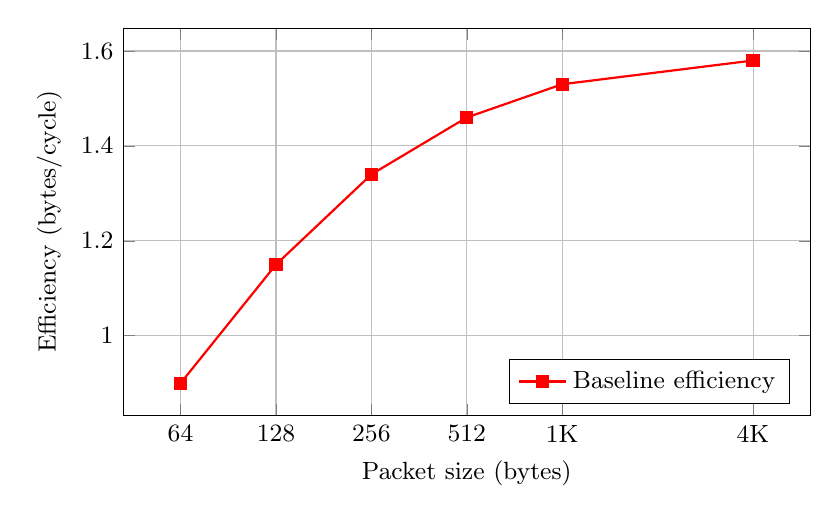
\begin{tikzpicture}
\begin{axis}[
    width=0.85\textwidth, height=6.5cm,
    xlabel={Packet size (bytes)}, ylabel={Efficiency (bytes/cycle)},
    xmode=log, log basis x=2,
    xtick={64,128,256,512,1024,4096},
    xticklabels={64,128,256,512,1K,4K},
    grid=major, legend pos=south east, font=\small
]
\addplot[mark=square*, thick, red] coordinates {(64,0.90) (128,1.15) (256,1.34) (512,1.46) (1024,1.53) (4096,1.58)};
\legend{Baseline efficiency}
\end{axis}
\end{tikzpicture}
\caption{Measured baseline efficiency versus packet size. Efficiency rises monotonically with packet size as the fixed PCIe and DMA overheads are amortised over more bytes, confirming the behaviour predicted by Equation~\ref{eq:efficiency}.}
\label{fig:baseline_efficiency}
\end{figure}

As predicted by Equation~\ref{eq:efficiency}, efficiency rises monotonically with packet size (\autoref{fig:baseline_efficiency}): a 64~B packet achieves only 0.90~bytes/cycle, while a 4~KB packet reaches 1.58~bytes/cycle -- a 76\% improvement in per-byte efficiency achieved purely by increasing packet size, with no change to the pipeline itself. This is the direct experimental confirmation of the small-packet inefficiency motivating this thesis (\autoref{sec:ch1_motivation}).

\subsection{Per-Stage Latency Breakdown}
\label{sec:ch7_breakdown}

The hardware latency monitor's breakdown estimator (\autoref{sec:ch5_latmon_impl}) decomposes each measured latency into its PCIe, DMA, and residual pipeline contributions using the closed-form estimate of Equation~\ref{eq:total_latency}. \autoref{tab:breakdown} reports this decomposition for all six baseline packet sizes.

\begin{table}[htbp]
\centering
\begin{tabular}{@{}rrrrr@{}}
\toprule
\textbf{Size (B)} & \textbf{PCIe (cyc)} & \textbf{DMA (cyc)} & \textbf{Other (cyc)} & \textbf{Total (cyc)} \\
\midrule
64   & 44   & 24   & 3 & 71   \\
128  & 68   & 40   & 3 & 111  \\
256  & 116  & 72   & 3 & 191  \\
512  & 212  & 136  & 3 & 351  \\
1024 & 404  & 264  & 3 & 671  \\
4096 & 1556 & 1032 & 3 & 2591 \\
\bottomrule
\end{tabular}
\caption{Per-stage latency breakdown (model-based estimate from \texttt{latency\_monitor}). ``PCIe'' and ``DMA'' each include the beat-transfer cycles their respective S\_SEND phase spends draining the packet buffer; ``Other'' is the residual contribution of the adapter, FIFO, and sink.}
\label{tab:breakdown}
\end{table}

The estimated PCIe and DMA contributions sum to within a constant 3 cycles of the measured total for every packet size in \autoref{tab:breakdown}, and that residual is identical across all six sizes. This confirms two things simultaneously: first, that the closed-form model of Equations~\ref{eq:pcie_latency}--\ref{eq:total_latency} correctly captures the dominant, size-dependent latency contributions of the implemented RTL; and second, that the pass-through stages between the DMA engine and the sink (the AXI-Stream adapter, an empty FIFO, and the sink's registered completion pulse) contribute a genuinely fixed, size-independent latency, with no hidden variable-length overhead that the model fails to account for.

%----------------------------------------------------------------------------------------

\section{Small-Packet Batching}
\label{sec:ch7_batching}

\autoref{tab:batching_results} compares Scenario~1 (batching enabled, four 64~B packets coalesced into one 256~B frame) against the corresponding baseline figure of sending the same four 64~B packets independently (Scenario~0's 64~B row, replicated four times and summed).

\begin{table}[htbp]
\centering
\begin{tabular}{@{}lrr@{}}
\toprule
\textbf{Configuration} & \textbf{Total Latency (cycles)} & \textbf{Efficiency (B/cycle)} \\
\midrule
4 $\times$ 64~B sent independently (baseline) & 284 & 0.90 \\
1 $\times$ 256~B batched frame (Scenario 1)    & 230 & 1.11 \\
\midrule
\textbf{Improvement} & \textbf{19.0\% latency reduction} & \textbf{1.25$\times$ efficiency} \\
\bottomrule
\end{tabular}
\caption{Batching four 64~B packets into one 256~B frame versus sending them independently, \texttt{BATCH\_COUNT=4}, \texttt{FIFO\_DEPTH=64}.}
\label{tab:batching_results}
\end{table}

\begin{figure}[htbp]
\centering
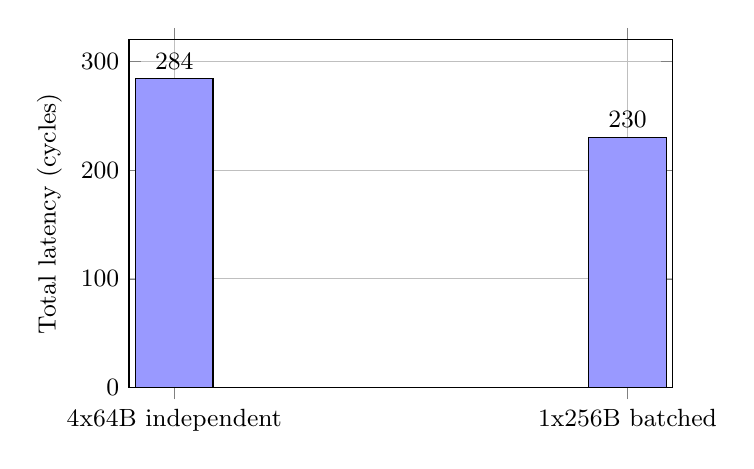
\begin{tikzpicture}
\begin{axis}[
    width=0.7\textwidth, height=6cm,
    ybar, bar width=28pt,
    ylabel={Total latency (cycles)},
    symbolic x coords={4x64B independent, 1x256B batched},
    xtick=data, nodes near coords, grid=major, font=\small,
    ymin=0, ymax=320
]
\addplot[fill=blue!40] coordinates {(4x64B independent,284) (1x256B batched,230)};
\end{axis}
\end{tikzpicture}
\caption{Total latency to deliver four 64~B packets' worth of payload (256~B): sent independently versus coalesced by the batching unit.}
\label{fig:batching_bar}
\end{figure}

The measured 230-cycle batch latency decomposes cleanly under Equation~\ref{eq:batch_inequality}: the first packet's own pipeline latency (approximately 71 cycles, from \autoref{tab:baseline_results}) plus three subsequent inter-packet gaps of approximately 53 cycles each (the time between one packet's PCIe stage completing and the next one's arriving, serialised by \texttt{pcie\_model}'s single-packet-in-flight design, \autoref{sec:ch5_pcie_fsm}), giving $71 + 3\times53 = 230$ cycles, matching the measurement exactly. Because the batching unit pays the PCIe base latency $T_{base}$ and DMA setup latency $T_{setup}$ (Equations~\ref{eq:pcie_latency}--\ref{eq:dma_latency}) only once for the whole 256~B frame rather than once per constituent 64~B packet, the 19\% reduction in \autoref{tab:batching_results} is a direct, measured instance of the amortisation inequality (Equation~\ref{eq:batch_inequality}) that motivated the batching unit's design (\autoref{sec:ch2_batching}, \autoref{sec:ch5_batching}).

One measurement subtlety is worth restating here (\autoref{sec:ch5_latmon_impl}): the latency monitor's per-packet \texttt{size\_store} table still records only 64~B for the batch's constituent injection events, since each \texttt{pkt\_inject} pulse is generated per individual packet by the testbench. Only because \texttt{stream\_sink} supplies the batch-aware \texttt{done\_size} (256~B, the true completed frame size) at the single completion event does the efficiency figure in \autoref{tab:batching_results} correctly reflect the coalesced transfer rather than understating it by a factor of four, as an earlier, uncorrected version of the monitor did (\autoref{tab:milestones}).

%----------------------------------------------------------------------------------------

\section{AXI-Stream FIFO Depth Sweep}
\label{sec:ch7_fifo}

Scenario~2 (\autoref{tab:tb_scenarios}) repeats the baseline packet-size sweep at \texttt{FIFO\_DEPTH} $\in \{16, 64, 256\}$ beats, first under the default always-ready sink and then under the optional rate-limited stall model (\autoref{sec:ch4_stream_sink}) that accepts one beat out of every four cycles.

\subsection{Always-Ready Sink}
\label{sec:ch7_fifo_always_ready}

Under the default always-ready sink, every one of the three FIFO depths reproduced the identical latency and efficiency figures already reported in \autoref{tab:baseline_results}, with the FIFO's peak occupancy never exceeding 1 beat and \texttt{fifo\_full} never asserted for any packet size, at any depth. This is the direct, expected consequence of the FIFO's first-word-fall-through read port (\autoref{sec:ch4_fifo}): with a consumer that drains every cycle it holds data, the FIFO is emptied on the same cycle a beat arrives, so it can never accumulate occupancy regardless of how deep it is configured to be, and \texttt{FIFO\_DEPTH} is consequently invisible to latency in this configuration. This null result is itself informative: it demonstrates that a FIFO-depth sweep is only a meaningful experiment once the datapath includes a genuine bottleneck downstream of the buffer, motivating the stalled-sink configuration below.

\subsection{Rate-Limited (Stalled) Sink}
\label{sec:ch7_fifo_stall}

\autoref{tab:fifo_stall} reports latency and peak FIFO occupancy for the same six packet sizes with the sink configured to accept only one beat in every four cycles (\texttt{SINK\_STALL\_READY=1}, \texttt{SINK\_STALL\_PERIOD=4}), at each of the three FIFO depths.

\begin{table}[htbp]
\centering
\begin{tabular}{@{}rrrrrrr@{}}
\toprule
& & \multicolumn{2}{c}{\textbf{Depth=16}} & \multicolumn{2}{c}{\textbf{Depth=64}} & \textbf{Depth=256} \\
\textbf{Size (B)} & \textbf{Latency (cyc)} & \textbf{Peak} & \textbf{Full?} & \textbf{Peak} & \textbf{Full?} & \textbf{Peak (Full?)} \\
\midrule
64   & 94   & 6  & no  & 6  & no  & 6 (no) \\
128  & 157  & 12 & no  & 12 & no  & 12 (no) \\
256  & 285  & 16 & yes & 24 & no  & 24 (no) \\
512  & 541  & 16 & yes & 48 & no  & 48 (no) \\
1024 & 1053 & 16 & yes & 64 & yes & 96 (no) \\
4096 & 4125 & 16 & yes & 64 & yes & 256 (yes) \\
\bottomrule
\end{tabular}
\caption{Latency and peak FIFO occupancy under a rate-limited sink (1 of every 4 cycles), at \texttt{FIFO\_DEPTH} $\in \{16, 64, 256\}$. Latency is identical across all three depths for every packet size; only the peak-occupancy and full-flag columns change.}
\label{tab:fifo_stall}
\end{table}

\begin{figure}[htbp]
\centering
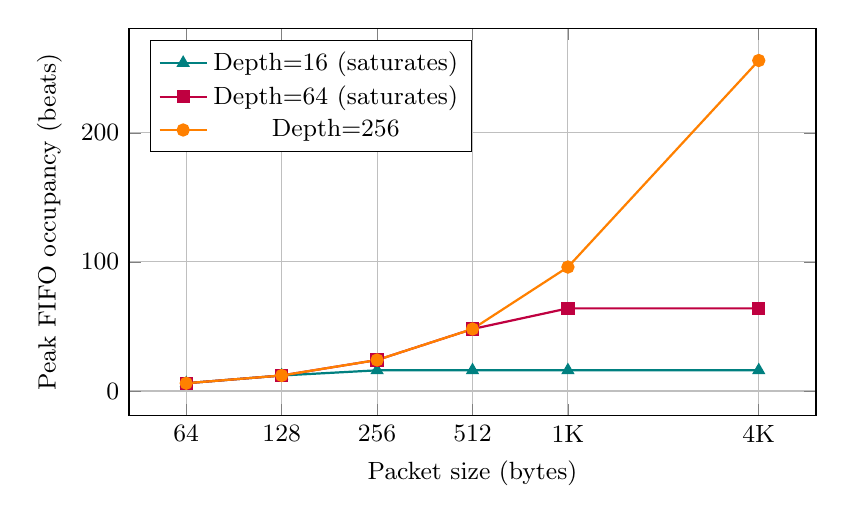
\begin{tikzpicture}
\begin{axis}[
    width=0.85\textwidth, height=6.5cm,
    xlabel={Packet size (bytes)}, ylabel={Peak FIFO occupancy (beats)},
    xmode=log, log basis x=2,
    xtick={64,128,256,512,1024,4096},
    xticklabels={64,128,256,512,1K,4K},
    grid=major, legend pos=north west, font=\small
]
\addplot[mark=triangle*, thick, teal] coordinates {(64,6) (128,12) (256,16) (512,16) (1024,16) (4096,16)};
\addplot[mark=square*, thick, purple] coordinates {(64,6) (128,12) (256,24) (512,48) (1024,64) (4096,64)};
\addplot[mark=*, thick, orange] coordinates {(64,6) (128,12) (256,24) (512,48) (1024,96) (4096,256)};
\legend{Depth=16 (saturates), Depth=64 (saturates), Depth=256}
\end{axis}
\end{tikzpicture}
\caption{Peak FIFO occupancy versus packet size under a rate-limited sink, at three FIFO depths. Shallower FIFOs saturate (hit \texttt{fifo\_full}) at smaller packet sizes; a deeper FIFO absorbs a larger packet before back-pressure engages.}
\label{fig:fifo_occupancy}
\end{figure}

The single most important observation in \autoref{tab:fifo_stall} is that \textbf{latency is identical across all three FIFO depths for every packet size} -- this is a correct, expected result, not an experimental artefact, and it is the reason \autoref{sec:ch3_queueing}'s distinction between buffering headroom and steady-state throughput was introduced analytically before this chapter presented the corresponding measurement. Once the sink's fixed drain rate (one beat every four cycles) becomes the pipeline's bottleneck, the total time required to push a fixed quantity of data through it is set entirely by that drain rate; a deeper upstream buffer can only change \emph{when} back-pressure begins reaching the producer, not the rate at which the single, continuously-flowing consumer ultimately drains the data. This is a direct hardware confirmation of the single-server queueing argument of \autoref{sec:ch3_queueing}.

What FIFO depth \emph{does} change, exactly as anticipated by \autoref{sec:ch4_fifo}, is how much of a given packet the FIFO can absorb before \texttt{fifo\_full} engages: the 16-entry (128~B) FIFO saturates for every packet of 256~B or larger, the 64-entry (512~B) FIFO saturates only from 1~KB upward, and the 256-entry (2~KB) FIFO saturates only for the 4~KB packet, since even a 2~KB buffer is smaller than a 4~KB payload (\autoref{fig:fifo_occupancy}). This is the correct, useful reading of a FIFO-depth sweep: it governs buffering headroom and how early back-pressure ripples upstream, not the completion latency of a single sustained flow once a fixed-rate consumer is the bottleneck. Making FIFO depth move the total latency figure itself would require a bursty, gapped traffic pattern -- so that a deeper buffer lets the producer run further ahead between bursts -- rather than the single continuous packet transfer studied here; this distinction is returned to as a direction for future work in \autoref{sec:ch8_future}.

%----------------------------------------------------------------------------------------

\section{Comparison with Prior Work}
\label{sec:ch7_comparison}

\autoref{sec:ch2_gap} identified Gu et al.~\cite{gu2025cooptimization} as the closest prior attempt at the small-packet PCIe DMA problem this thesis addresses, and adopted it as the baseline to compare against. A direct, apples-to-apples number is not possible: Gu et al. measure real Gen3 traffic on a Xilinx VC709 board in GB/s and microseconds under a randomised data-centre-like packet mix, while this thesis measures a behavioural RTL model in simulated clock cycles under directed packet-size sweeps (\autoref{Chapter6}). What \emph{can} be compared fairly is the mechanism each uses to get its improvement, where in the system that mechanism sits, and whether the improvement can be attributed to a specific cause or only observed as an aggregate change. \autoref{tab:comparison} summarises this.

\begin{table}[htbp]
\centering
\begin{tabular}{@{}p{2.3cm}p{3.4cm}p{3.6cm}p{3.6cm}@{}}
\toprule
\textbf{Study} & \textbf{Where the fix is applied} & \textbf{Reported improvement} & \textbf{Latency attributable to a specific stage?} \\
\midrule
Gu et al.~\cite{gu2025cooptimization} & Linux driver (descriptor prefetch) + PCIe config-space register (extended tag) + host CPU (multicore dispatch) & 123--136\% bandwidth, 15.1--24.0\% latency, randomised small-packet mix, real VC709/XDMA hardware & No -- three mechanisms are enabled together; the paper reports one combined GB/s and $\mu$s figure \\
Kavianipour \& B{\"o}hm~\cite{kavianipour2012high} & Host-side buffer merging before the DMA call & Up to 1080~MB/s for merged/vectored writes vs.\ much lower for un-merged small (12~B) buffers & No -- throughput only, no latency breakdown \\
This thesis & \texttt{batching\_unit}, a single RTL block on the AXI4-Stream side, upstream of \texttt{pcie\_model}/\texttt{dma\_model} & 19.0\% latency reduction, 1.25$\times$ efficiency, for four 64~B packets coalesced into one 256~B frame (\autoref{tab:batching_results}) & Yes -- the \texttt{latency\_monitor} breakdown (\autoref{tab:breakdown}) attributes the saving to paying $T_{base}$ and $T_{setup}$ once instead of four times \\
\bottomrule
\end{tabular}
\caption{Mechanism-level comparison with the two closest prior PCIe-DMA studies. Absolute GB/s and $\mu$s figures from real hardware are not directly comparable to simulated-cycle figures from a behavioural RTL model; the comparison here is of mechanism and attributability, not of raw magnitude.}
\label{tab:comparison}
\end{table}

Two things follow from this comparison. First, the part of this thesis's architecture responsible for the measured improvement is specifically the \texttt{batching\_unit} stage (\autoref{sec:ch4_batching_unit}, \autoref{sec:ch5_batching}): it is the only block that changes between the baseline and batched configurations of \autoref{sec:ch7_batching}, so the entire 19\% reduction is attributable to it and to nothing else in the pipeline. Gu et al.'s 15--24\% latency improvement, by contrast, is the joint effect of a modified host driver, a reconfigured PCIe extended-tag field, and multicore dispatch, so their paper cannot say how much of it comes from any one change. Second, the two results are not really in competition: Gu et al.'s techniques operate on the host and PCIe-configuration side of the link, while the batching unit operates entirely on the AXI4-Stream side, before a packet ever reaches \texttt{pcie\_model}. Nothing in principle stops the two from being combined -- the batching unit would simply present the descriptor-prefetch-augmented driver with fewer, larger transfers to prefetch for -- but demonstrating that combination is left as future work (\autoref{sec:ch8_future}), since it would require replacing the behavioural \texttt{pcie\_model} of this thesis with the real XDMA/driver stack that Gu et al. used, which \autoref{sec:ch8_limitations} identifies as a limitation of the current implementation.

%----------------------------------------------------------------------------------------

% \section{Discussion}
% \label{sec:ch7_discussion}

% Taken together, the results of this chapter support three conclusions. First, the analytical fixed-plus-proportional latency model of \autoref{sec:ch3_latency_model} is not merely a simplifying assumption but an accurate description of the implemented RTL: \autoref{tab:breakdown} shows the model-based PCIe and DMA estimates matching the hardware-measured total to within a constant 3-cycle residual across a 64-fold range of packet sizes. Second, the small-packet inefficiency this thesis set out to quantify is substantial and measurable in cycle-accurate simulation, not just in principle: a 64~B transfer achieves only 57\% of the per-byte efficiency of a 4~KB transfer (\autoref{tab:baseline_results}), and the batching unit recovers a meaningful fraction of that gap -- a 19\% latency reduction for a representative 4-packet burst -- using a mechanism whose correctness was verified directly against its own simulation diagnostics (\autoref{sec:ch6_milestones}) rather than assumed from the design alone. Third, the FIFO-depth results (\autoref{tab:fifo_stall}) demonstrate a distinction -- between buffering headroom and steady-state single-flow latency -- that is easy to conflate when sizing a DMA buffer from bandwidth figures alone, and that this thesis's testbed makes directly and unambiguously measurable by contrasting the always-ready and rate-limited sink configurations.
 
% Chapter 8

\chapter{Conclusions and Future Work}

\label{Chapter8}

\lhead{Chapter 8. \emph{Conclusions and Future Work}}

\section{Conclusions}
\label{sec:ch8_conclusions}

This thesis set out to quantify, and partially mitigate, the disproportionately high per-byte latency that small packets incur when moved across a PCIe-AXI DMA streaming datapath. Starting from the observation that both PCIe transaction-layer processing and DMA descriptor handling impose a largely fixed, size-independent cost per transfer (\autoref{Chapter3}), a seven-stage, cycle-accurate SystemVerilog model of such a datapath was designed and implemented (\autoref{Chapter4}, \autoref{Chapter5}), instrumented with a hardware latency monitor that measures every packet's latency directly from simulated RTL signals rather than from a software proxy (\autoref{sec:ch4_latency_monitor}), and exercised with a directed testbench across packet sizes from 64~B to 4~KB and across three FIFO depths under two consumer models (\autoref{Chapter6}).

The resulting measurements (\autoref{Chapter7}) confirm the thesis's central hypothesis quantitatively: baseline efficiency rises from 0.90~bytes/cycle at 64~B to 1.58~bytes/cycle at 4~KB (\autoref{tab:baseline_results}), and this behaviour is explained, to within a constant 3-cycle residual across every packet size tested, by the closed-form PCIe-plus-DMA latency model derived in \autoref{sec:ch3_latency_model} (\autoref{tab:breakdown}). A packet-batching unit designed specifically to amortise this fixed overhead across multiple small packets (\autoref{sec:ch5_batching}) was shown to reduce the total latency of transferring four 64~B packets from 284 cycles (sent independently) to 230 cycles (coalesced into one 256~B frame) -- a 19\% reduction, obtained by paying the fixed PCIe and DMA overhead once instead of four times (\autoref{sec:ch7_batching}). A complementary FIFO-depth sweep under a rate-limited consumer showed that buffer depth governs buffering headroom -- how much of a packet the FIFO can absorb before back-pressure engages -- but, once a fixed-rate consumer is the pipeline's bottleneck, does not itself change the steady-state completion latency of a single continuous transfer (\autoref{sec:ch7_fifo_stall}), a distinction that is easy to overlook when sizing DMA buffers from bandwidth specifications alone.

\section{Research Contributions}
\label{sec:ch8_contributions}

The specific contributions of this thesis are:

\begin{enumerate}
    \item A closed-form, packet-size-parameterised latency model (Equations~\ref{eq:pcie_latency}--\ref{eq:total_latency}) for a PCIe transaction layer and a descriptor-based DMA engine, validated directly against cycle-accurate hardware measurements across a 64-fold range of packet sizes with a constant, fully-accounted-for residual.
    \item An open, synthesisable, seven-stage SystemVerilog implementation of a PCIe-AXI DMA streaming pipeline (\texttt{pcie\_model}, \texttt{dma\_model}, \texttt{axi\_mm2s\_adapter}, \texttt{axis\_fifo}, \texttt{batching\_unit}, \texttt{stream\_sink}, \texttt{latency\_monitor}), together with a directed, self-checking testbench, that can be re-parameterised and re-simulated to study configurations beyond those reported in this thesis.
    \item A hardware, in-design latency-measurement block that timestamps packet injection and completion events directly in RTL and decomposes every measured latency into its PCIe, DMA, and residual pipeline contributions, avoiding the software-side reference-point misalignment that produced a spurious constant offset in an earlier version of the testbench (\autoref{sec:ch6_milestones}).
    \item A small-packet batching unit, implemented as a zero-buffering, online pass-through stage, with a measured 19\% latency reduction and $1.25\times$ efficiency improvement for a representative four-packet burst, demonstrated using the same RTL and testbench as the un-batched baseline so that the comparison isolates the effect of a single enable bit.
    \item An experimental demonstration, using an always-ready and a rate-limited consumer model of the same FIFO, that clearly separates the buffering-headroom role of FIFO depth from its (in this workload, negligible) effect on steady-state single-flow completion latency.
\end{enumerate}

\section{Limitations}
\label{sec:ch8_limitations}

The present model and its evaluation have several limitations, acknowledged here so that the results of \autoref{Chapter7} are interpreted with the correct scope.

\begin{itemize}
    \item \textbf{Single packet in flight.} Both \texttt{pcie\_model} and \texttt{dma\_model} buffer and process one packet at a time (\autoref{sec:ch5_pcie_fsm}, \autoref{sec:ch5_dma_fsm}), matching the testbench's sequential injection pattern but not modelling pipelined, overlapping in-flight transactions, credit-based multi-outstanding-request behaviour, or PCIe multi-lane/multi-virtual-channel effects, all of which a production PCIe root complex or endpoint would exploit to improve small-packet throughput beyond what a single-packet-at-a-time model can show.
    \item \textbf{Behavioural, not RTL-synthesised-and-timed, PCIe and DMA models.} \texttt{pcie\_model} and \texttt{dma\_model} are parameterised behavioural approximations of PCIe and DMA timing (\autoref{sec:ch3_pcie}, \autoref{sec:ch3_dma}), not a synthesised PCIe hard IP or a commercial DMA IP core such as \cite{xilinx2021axidma, xilinx2021pcieintblock}; their fixed and per-byte constants were chosen to be representative of typical Gen3-class timing rather than measured from a specific silicon implementation.
    \item \textbf{Batching corner case.} As noted in \autoref{sec:ch5_batching}, the batching unit will not flush an incomplete final batch that is not followed by a further \texttt{tlast}; the testbench's batching scenario always injects a complete batch of \texttt{BATCH\_COUNT} packets, so this case is not exercised in this thesis's results, but it would need to be addressed (e.g. with an explicit external flush signal) before the unit could be deployed against an arbitrary, potentially bursty packet stream.
    \item \textbf{One workload pattern per FIFO-depth experiment.} The FIFO-depth sweep of \autoref{sec:ch7_fifo} drives one continuous packet through the pipeline at a time; as discussed in \autoref{sec:ch7_fifo_stall}, this is precisely the workload pattern under which FIFO depth does not affect steady-state latency, and a bursty, multi-packet-in-flight traffic pattern would be needed to observe the buffering benefit that FIFO depth is, in general, provisioned for.
    \item \textbf{No physical validation.} All results in this thesis are obtained from RTL simulation in Vivado \texttt{xsim} \cite{xilinx2022vivadosim}; no FPGA bring-up, hardware-in-the-loop measurement, or comparison against a real PCIe link's measured latency was performed.
\end{itemize}

\section{Scope for Future Work}
\label{sec:ch8_future}

Several extensions follow directly from the limitations above and from observations made during the analysis of \autoref{Chapter7}:

\begin{enumerate}
    \item \textbf{Multi-packet-in-flight modelling.} Extending \texttt{pcie\_model} and \texttt{dma\_model} to pipeline or overlap multiple in-flight packets, rather than processing one at a time, would allow the model to capture the throughput gains a real multi-outstanding-transaction PCIe link achieves and would be a prerequisite for studying burst/gapped traffic patterns under which FIFO depth is expected to affect latency directly (\autoref{sec:ch7_fifo_stall}).
    \item \textbf{Bursty workload FIFO study.} Re-running the FIFO-depth sweep of \autoref{sec:ch7_fifo} under a workload of bursts separated by idle gaps, rather than one continuous transfer, would directly test the hypothesis raised in \autoref{sec:ch7_discussion} that FIFO depth's real benefit is letting the producer run ahead between bursts.
    \item \textbf{Adaptive batching.} The present batching unit uses a fixed \texttt{BATCH\_COUNT} and \texttt{BATCH\_TIMEOUT} (\autoref{sec:ch5_batching}); an adaptive policy that adjusts these based on observed packet arrival rate could trade off the latency-per-packet cost of waiting to fill a batch against the throughput benefit of a larger one, and would need its own latency-vs-arrival-rate characterisation using the same measurement infrastructure built in this thesis.
    \item \textbf{Validation against a commercial DMA/PCIe IP core.} Replacing the behavioural \texttt{pcie\_model} and \texttt{dma\_model} with a synthesised instance of a commercial core such as the AMD-Xilinx AXI DMA IP or UltraScale+ PCIe integrated block \cite{xilinx2021axidma, xilinx2021pcieintblock}, driven by the same testbench and latency monitor, would validate how closely this thesis's behavioural constants correspond to a real implementation's timing.
    \item \textbf{Hardware bring-up.} Deploying the design on an FPGA connected to a real PCIe root complex and comparing host-measured round-trip latency against the simulated figures of \autoref{Chapter7} would close the loop between this thesis's simulation-only results and physically measured behaviour.
\end{enumerate}

%----------------------------------------------------------------------------------------
%	THESIS CONTENT - APPENDICES
%----------------------------------------------------------------------------------------

\addtocontents{toc}{\vspace{2em}} % Add a gap in the Contents, for aesthetics

\appendix % Cue to tell LaTeX that the following 'chapters' are Appendices

% Include the appendices of the thesis as separate files from the Appendices folder
% Uncomment the lines as you write the Appendices

% Appendix A

\chapter{Package Parameters and Representative Simulation Output}

\label{AppendixA}

\lhead{Appendix A. \emph{Package Parameters and Representative Simulation Output}}

This appendix lists the complete set of configuration parameters exported by \texttt{pcie\_axi\_pkg} (\autoref{sec:ch4_sideband}) and reproduces a representative excerpt of the simulator's \texttt{[RESULT]} output for the baseline scenario (\autoref{sec:ch7_baseline}), for reference alongside the summarised tables of \autoref{Chapter7}.

\section{Complete Package Parameter Listing}
\label{sec:appA_params}

\begin{table}[htbp]
\centering
\begin{tabular}{@{}lrl@{}}
\toprule
\textbf{Parameter} & \textbf{Default} & \textbf{Description} \\
\midrule
\texttt{DATA\_WIDTH}              & 64   & AXI-Stream data bus width (bits) \\
\texttt{STRB\_WIDTH}               & 8    & \texttt{DATA\_WIDTH/8} (bytes per beat) \\
\texttt{PKT\_SIZE\_W}              & 13   & Packet byte-length field width (0--8191 B) \\
\texttt{PKT\_ID\_W}                & 8    & Packet tag/ID field width (0--255) \\
\texttt{ADDR\_WIDTH}               & 32   & AXI memory-mapped address width \\
\texttt{PCIE\_BASE\_LATENCY}        & 20   & PCIe fixed per-TLP overhead (cycles) \\
\texttt{PCIE\_PER\_DW\_LATENCY}     & 1    & PCIe overhead per 4-byte DWORD (cycles) \\
\texttt{DMA\_SETUP\_CYCLES}         & 8    & DMA descriptor-fetch overhead (cycles) \\
\texttt{DMA\_BYTES\_PER\_CYC}       & 8    & DMA effective transfer rate (bytes/cycle) \\
\texttt{FIFO\_DEPTH\_DEFAULT}       & 64   & AXI-Stream FIFO depth (beats) \\
\texttt{BATCH\_COUNT\_DEFAULT}      & 4    & Packets coalesced per batch \\
\texttt{BATCH\_TIMEOUT\_DEFAULT}    & 64   & Idle cycles before forced batch flush \\
\texttt{SINK\_STALL\_EN\_DEFAULT}   & 0    & Consumer back-pressure model enable \\
\texttt{SINK\_STALL\_PERIOD\_DEFAULT}& 4   & Consumer stall period (cycles) \\
\texttt{SINK\_STALL\_READY\_DEFAULT}& 1    & Consumer ready cycles per period \\
\texttt{TIMESTAMP\_WIDTH}          & 32   & Latency-monitor cycle-counter width (bits) \\
\texttt{MAX\_PACKETS}              & 256  & Max in-flight packets tracked by the monitor \\
\bottomrule
\end{tabular}
\caption{Complete parameter listing from \texttt{pcie\_axi\_pkg.sv}.}
\label{tab:appA_params}
\end{table}

\section{Representative Simulator Output}
\label{sec:appA_output}

The excerpt below reproduces the \texttt{[RESULT]} table format emitted by the testbench (\autoref{sec:ch6_testbench}) for the baseline scenario (\texttt{TB\_SCENARIO=0}, \texttt{FIFO\_DEPTH=64}), summarised in \autoref{tab:baseline_results}.

\begin{verbatim}
[RESULT] ================================================================
[RESULT]  PCIe-AXI DMA Latency Simulation  |  Config: BASELINE,FIFO=64
[RESULT] ================================================================
[RESULT]  PKT_ID | SIZE (B) | LATENCY (cyc) | EFFICIENCY (B/cyc) | FIFO_PEAK | FULL?
[RESULT] ----------------------------------------------------------------
[RESULT]       0 |       64 |            71 |               0.90 |         1 |    no
[RESULT]       1 |      128 |           111 |               1.15 |         1 |    no
[RESULT]       2 |      256 |           191 |               1.34 |         1 |    no
[RESULT]       3 |      512 |           351 |               1.46 |         1 |    no
[RESULT]       4 |     1024 |           671 |               1.53 |         1 |    no
[RESULT]       5 |     4096 |          2591 |               1.58 |         1 |    no
[RESULT] ----------------------------------------------------------------
[RESULT]  Total packets received: 6
[RESULT] ================================================================
\end{verbatim}

The corresponding hardware latency-monitor summary, printed once at the end of simulation from the \texttt{final} block of \texttt{latency\_monitor} (\autoref{sec:ch4_latency_monitor}), is:

\begin{verbatim}
[latmon] ================================================
[latmon]         LATENCY MONITOR SUMMARY
[latmon] ================================================
[latmon]  Packets measured : 6
[latmon]  Min latency      : 71     cycles
[latmon]  Max latency      : 2591   cycles
[latmon]  Avg latency      : 664.3  cycles
[latmon]  Total bytes      : 6080   bytes
[latmon]  Avg efficiency   : 1.53   B/cyc
[latmon]  Eff throughput   : 152.5  MB/s (100MHz)
[latmon] ================================================
\end{verbatim}


\addtocontents{toc}{\vspace{2em}} % Add a gap in the Contents, for aesthetics

\backmatter

%----------------------------------------------------------------------------------------
%	BIBLIOGRAPHY
%----------------------------------------------------------------------------------------
\nocite{*}
\label{Bibliography}

\lhead{\emph{Bibliography}} % Change the page header to say "Bibliography"

\bibliographystyle{ieeetr} % Use the "custom" BibTeX style for formatting the Bibliography

\bibliography{Bibliography} % The references (bibliography) information are stored in the file named "Bibliography.bib"

\end{document}  
